\documentclass[12pt]{article}
\usepackage{fullpage,islsymb,graphicx,makeidx}
\makeindex

\def\cvxver{1.1\xspace}
\def\cvxbuild{570\xspace}
\DefineVerbatimEnvironment{code2}{Verbatim}{tabsize=0,xleftmargin=0.5in,numbers=left,firstnumber=last,commandchars=\!\{\}}

\def\Rank{\operatorname*{\textbf{Rank}}}
\newcommand{\symm}{{\mbox{\bf S}}}  % symmetric matrices
\newcommand{\herm}{{\mbox{\bf H}}}  % Hermitian matrices
\newcommand{\lorentz}{{\mbox{\bf Q}}}  % lorentz cone
\newcommand{\ones}{\mathbf 1}
\setcounter{tocdepth}{2}

\title{\cvx Users' Guide\\\large for \cvx version \cvxver (build \cvxbuild)}
\author{Michael Grant\\\texttt{mcgrant@stanford.edu} 
\and Stephen Boyd\\\texttt{boyd@stanford.edu}
\and Yinyu Ye\\\texttt{yyye@stanford.edu}}
\bibliographystyle{alpha}

\begin{document}
\maketitle
\clearpage
\tableofcontents
\clearpage

\section{Introduction}

\subsection{What is \cvx?}
\index{cvx@{\cvx}}
\index{disciplined convex programming|see{DCP}}
\index{DCP}
\index{linear!program|see{LP}}
\index{LP}
\index{quadratic program|see{QP}}
\index{QP}
\index{second-order cone program|see{SOCP}}
\index{SOCP}
\index{geometric program|see{GP}}
\index{GP}
\index{semidefinite program|see{SDP}}
\index{SDP}
\index{Matlab}

\cvx is a modeling system for \emph{disciplined convex programming}. 
Disciplined convex programs, or DCPs, are convex optimization problems 
that are described using a limited set of construction rules, which
enables them to be analyzed and solved efficiently.  \cvx can solve 
standard problems such as linear programs (LPs), quadratic programs (QPs),
second-order cone programs (SOCPs), and semidefinite programs (SDPs);
but compared to directly using a solver for one or these types of problems,
\cvx can greatly simplify the task of specifying the problem.
\cvx can also solve much more complex convex optimization problems,
including many involving nondifferentiable functions, such as $\ell_1$
norms.
You can use \cvx to conveniently formulate and solve
constrained norm minimization, entropy maximization,
determinant maximization, and many other problems.

To use \cvx effectively, you need to know at least a bit about 
convex optimization.
For background on convex optimization,
see the book \emph{Convex Optimization} \cite{BV:04}, available on-line
at \url{www.stanford.edu/~boyd/cvxbook/}, or the 
Stanford course EE364A, available at
\url{www.stanford.edu/class/ee364a/}.

\cvx is implemented in Matlab \cite{MATLAB}, effectively
turning Matlab into an optimization modeling language.
Model specifications are constructed using common Matlab
operations and functions, and standard Matlab code can be
freely mixed with these specifications. This combination
makes it simple to perform the calculations
needed to form optimization problems, or to process the
results obtained from their solution. For example, it is easy
to compute an optimal trade-off curve
by forming and solving a family of optimization problems
by varying the constraints. As another example, \cvx can
be used as a component of a larger system that uses convex
optimization, such as a branch and bound method,
or an engineering design framework.

\cvx also provides special modes to simplify 
the construction of problems
from two specific problem classes. In \emph{SDP mode}, \cvx applies
a matrix interpretation to the inequality operator, so that
\emph{linear matrix inequalities} (LMIs) and SDPs may be expressed
in a more natural form. In \emph{GP mode}, \cvx accepts all of the
special functions and combination rules of geometric programming,
including monomials, posynomials, and generalized posynomials,
and transforms such problems into convex form
so that they can be solved efficiently.
For background on geometric programming, see the tutorial paper
\cite{BKVH:05}, available
at \url{www.stanford.edu/~boyd/papers/gp_tutorial.html}.
\index{SDP!mode}
\index{GP!mode}

\index{YALMIP}
\index{AMPL}
\index{GAMS}
\index{python}
\cvx was designed and implemented by Michael Grant, with input
from Stephen Boyd and Yinyu Ye \cite{GBY}. It
incorporates ideas from earlier work by 
L\"{o}fberg \cite{YALMIP}, 
Dahl and Vandenberghe \cite{CVXOPT}, 
Crusius \cite{Cru:02}, 
Wu and Boyd \cite{SDPSOL},
and many others.
The modeling language follows
the spirit of AMPL \cite{AMPL} or GAMS \cite{GAMS}; unlike
these packages, however, \cvx was designed from the beginning 
to fully exploit convexity.
The specific method for implementing \cvx in Matlab
draws heavily from YALMIP \cite{YALMIP}. We also hope
to develop versions of \cvx for other platforms in the future.

\subsection{What is disciplined convex programming?}
\label{sec:what-is-dcp}
\index{disciplined convex programming|see{DCP}}
\index{DCP}

\emph{Disciplined convex programming} is
a methodology for constructing convex optimization problems
proposed by Michael Grant, Stephen Boyd, and Yinyu Ye \cite{GBY,Gra:04}.
%The name was chosen to communicate the treatment of convex
%programming as a distinct discipline, one in which convexity is an
%advance requirement. 
It is meant to support the formulation and
construction of optimization problems that the user 
intends \emph{from the outset} to be convex.
\index{DCP!ruleset}
Disciplined convex programming imposes a
set of conventions or rules, which we call the \emph{DCP ruleset}.
Problems which adhere to the ruleset can be rapidly and automatically
verified as convex and converted to solvable form.
Problems that violate the ruleset are rejected, even 
when the problem is convex.
That is not to say that such problems cannot be solved using DCP; they
just need to be rewritten in a way that conforms to the DCP ruleset.

A detailed description of the DCP ruleset is given in \S\ref{sec:rules},
and it is important for anyone who intends to actively use
\cvx to understand it.
The ruleset is simple 
to learn, and is drawn from basic principles of convex analysis.
In return for accepting the restrictions imposed by the ruleset,
we obtain considerable benefits, such as automatic conversion of
problems to solvable form, and full support for nondifferentiable 
functions. 
In practice, we have found that
disciplined convex programs closely resemble
their natural mathematical forms.

\subsection{About this version}
\label{sec:version}
\index{version information}
\index{SeDuMi}
\index{SDPT3}
\index{MOSEK}
\index{LP}
\index{SDP}
\index{SOCP}
\index{CVXOPT}
\paragraph{Supported solvers.}
This version of \cvx supports two core solvers, SeDuMi
\cite{Stu:99} and SDPT3 \cite{SDPT3}, which is the default.
Future versions of \cvx may support other solvers, such as
MOSEK \cite{MOSEK} or CVXOPT \cite{CVXOPT}.
SeDuMi and SDPT3 are open-source interior-point solvers written in Matlab for 
LPs, SOCPs, SDPs, and combinations thereof.

\paragraph{Problems handled exactly.}
\cvx will convert the specified problem to an LP, SOCP, or SDP,
when all the functions in the problem specification can be
represented in these forms.
This includes a wide variety of functions, such as minimum and
maximum, absolute value, quadratic forms, 
the minimum and maximum eigenvalues of a symmetric matrix,
power functions $x^p$, and $\ell_p$ norms (both for $p$ rational).
%A few obscure functions have also been included, 
%such as the sum of the $k$ largest entries of a vector, and the
%convex envelope of a nonconvex polynomial.

\paragraph{Problems handled with (good) approximations.}
For a few functions, \cvx will make a (good) approximation to transform the
specified problem to one that can be handled by a combined 
LP, SOCP, and SDP solver.
For example, when a power function or $\ell_p$-norm is used, with 
non-rational exponent $p$, \cvx replaces $p$ with a nearby rational.
The log of the normal cumulative distribution $\log \Phi(x)$ is
replaced with an SDP-compatible approximation.

\paragraph{Problems handled with successive approximation.}
This version of \cvx adds support for a number of functions that cannot
be exactly represented via LP, SOCP, or SDP, including 
log, exp, log-sum-exp $\log (\exp x_1+ \cdots + \exp x_n)$,
entropy, and Kullback-Leibler divergence.
These problems are handled by solving a sequence (typically just a handful)
of SDPs, which yields the solution to the full accuracy of the core solver.
On the other hand, this technique can be 
\emph{substantially slower}
than if the core solver directly handled such functions.
The successive approximation method is briefly described in
Appendix \ref{sec:succ-approx}. Geometric problems are now solved in
this manner as well; in previous versions, an approximation was made.

Ultimately, we will interface \cvx to a solver with native support for 
such functions, which result in a large speedup in solving problems
with these functions.
Until then, users should be aware that problems involving these functions
can be slow to solve using the current version of \cvx.
For this reason, when one of these functions is used, the user will be 
warned that the successive approximate technique will be used.

We emphasize that most users do not need 
to know how \cvx handles their problem; what matters is what functions
and operations can be handled.
For a full list of functions supported by \cvx, 
see Appendix \ref{s-functions}, or use the online help function by typing
\verb+help cvx/builtins+ 
(for functions already in Matlab, such as \verb+sqrt+ or \verb+log+)
or \verb+help cvx/functions+
(for functions not in Matlab, such as \verb+lambda_max+).

\subsection{Feedback}
\label{sec:feedback}
\index{feedback}
\index{bug report}

Please contact Michael Grant (\texttt{mcgrant@stanford.edu}) 
or Stephen Boyd (\texttt{boyd@stanford.edu}) with 
your comments. If you discover what you think is a bug, 
please include the following in your communication,
so we can reproduce and fix the problem:
\begin{itemize}
\item the \cvx model and supporting data that caused the error
\item a copy of any error messages that it produced
\item the \cvx version number and build number
\item the version number of Matlab that you are running
\item the name and version of the operating system you are using
\end{itemize}
The latter three items can all be discovered by typing
\begin{code}
	cvx_version
\end{code}
at the MATLAB command prompt; simply copy its output
into your email message.

\subsection{What \cvx is \emph{not}}

%\begin{itemize}
%\item 
\cvx is \emph{not} meant to be a tool for checking if your problem
is convex.  
You need to know a bit about 
convex optimization to effectively use \cvx; otherwise you are the proverbial
monkey at the typewriter, hoping to (accidently) type in a valid disciplined
convex program.

On the other hand, if \cvx accepts your problem, you can be sure
it is convex.
In conjunction with a course on (or self study of) convex optimization,
\cvx (especially, its error messages) can be very helpful in learning
some basic convex analysis.
While \cvx will attempt to give helpful error messages when
you violate the DCP ruleset, it can sometimes give quite obscure error
messages.  

%\item
\cvx is \emph{not} meant
for very large problems, so if your problem is very large
(for example, a large image processing problem), \cvx is unlikely to
work well (or at all).
For such problems you will likely need to directly call a solver,
or to develop your own methods, to get the efficiency you need.

For such problems \cvx can play an important role, however.  Before
starting to develop a specialized large-scale method, you can use \cvx
to solve scaled-down or simplified versions of the problem, to rapidly
experiment with exactly what problem you want to solve.
For image reconstruction, for example, you might use \cvx to experiment
with different problem formulations on $50 \times 50$ pixel images.

\cvx \emph{will}
solve many medium and large scale problems, provided they
have exploitable structure (such as sparsity), and you 
avoid \verb+for+ loops, which can be slow in Matlab, and functions
like log and exp that require successive approximation.
If you encounter difficulties in solving large problem instances,
please do contact us; we may be able to suggest
an equivalent formulation that \cvx can process more efficiently.

%Our goal in the design of \cvx is to greatly simplify the 
%specification and solution of convex optimization problems. 
%One indication of the progress we have made
%towards this goal is the ease with which some users 
%have encountered the limits
%of the software's performance, by creating models that are too 
%large for \cvx to solve.

%Such limits are unavoidable due to a number of factors, including
%the finite
%resources of a typical PC, the overhead imposed by the Matlab 
%environment,
%and the general-purpose design of the underlying numerical solver.
%Thus while \cvx should perform
%well for medium scale problems and many structured large-scale 
%problems, it may
%encounter difficulties when scaling to large problem instances.

%Despite this advance warning, 
%we would still greatly appreciate if you would send
%us feedback if you do encounter limits like these.
%In some cases, such reports have led to genuine improvements in the
%implementation of \cvx that have
%increased its capacity or performance. 
%\end{itemize}

\newpage
\section{A quick start}
\label{sec:quickstart}

\index{cvx_begin@\texttt{cvx\_begin}}
\index{cvx_end@\texttt{cvx\_end}}
\index{examples}
Once you have installed \cvx (see \S\ref{s-installing}), you can
start using it by entering a \cvx \emph{specification} into a
Matlab script or function, or directly from the command prompt.
To delineate \cvx specifications from surrounding Matlab code,
they are preceded with the statement
\verb@cvx_begin@ and followed with the statement
\verb@cvx_end@. A specification can
include any ordinary Matlab statements, as well as
special \cvx-specific commands for declaring primal and dual 
optimization variables and specifying constraints and
objective functions.

Within a \cvx specification, optimization variables have no numerical
value; instead, they are special Matlab objects.   
This enables Matlab to distinguish
between ordinary commands and \cvx objective
functions and constraints. As Matlab reads a \cvx specification,
it builds an internal representation of the
optimization problem. If it encounters a
violation of the rules of disciplined convex programming
(such as an invalid use of a composition rule or an invalid
constraint), an error message is generated.
When Matlab reaches 
the \verb@cvx_end@ command, it completes the conversion of
the \cvx specification to a canonical form,
and calls the underlying core solver to solve it.
%(SeDuMi or SDPT3, in this version).

If the optimization is successful,
the optimization variables declared in the \cvx specification
are converted from objects to ordinary Matlab numerical values
that can be used in any further Matlab calculations. In addition,
\cvx also assigns a few other related Matlab variables.
One, for example, gives the status of the problem (\ie, whether an
optimal solution was found, or the problem was determined to be 
infeasible or unbounded).  Another gives the optimal value
of the problem. Dual variables can also be assigned.

This processing flow will become more clear as we introduce
a number of simple examples. We invite the reader to actually follow
along with these examples in Matlab, by running the \verb@quickstart@
script found in the \verb@examples@ subdirectory of the \cvx distribution. 
For example,
if you are on Windows, and you have installed the \cvx distribution
in the directory \verb@D:\Matlab\cvx@, then you would type
\begin{code}
	cd D:\Matlab\cvx\examples
	quickstart
\end{code}
at the Matlab command prompt.
The script will automatically print key excerpts of its code, and
pause periodically so you can examine its output. (Pressing ``Enter''
or ``Return'' resumes progress.) 
The line numbers accompanying the code excerpts in this
document correspond to the line numbers in the file \verb@quickstart.m@.

\subsection{Least-squares}
\label{sec:leastsquares}
\index{least squares}

We first consider the most basic convex optimization problem,
least-squares.
In a least-squares problem, we seek $x \in \R^n$
that minimizes $\|Ax-b\|_2$, where $A\in \R^{m \times n}$ is
skinny and full rank (\ie, $m\geq n$ and $\Rank (A)=n$).
Let us create some test problem data for $m$, $n$, $A$, and $b$ in Matlab:
\begin{code2}[firstnumber=15]
	m = 16; n = 8;
	A = randn(m,n);
	b = randn(m,1);
\end{code2}
(We chose small values of $m$ and $n$ to keep the output readable.)
Then the least-squares solution  $x=(A^TA)^{-1}A^Tb$ is easily
computed using the backslash operator: 
\begin{code2}[firstnumber=20]
	x_ls = A \ b;
\end{code2}
\index{variable@\texttt{variable}}
\index{minimize@\texttt{minimize}}
\index{norm@\texttt{norm}}
\index{objective function}
\index{function!objective}
Using \cvx, the same problem can be solved as follows:
\begin{code2}[firstnumber=23]
	cvx_begin			!label{code:beg}
	    variable x(n);		!label{code:var}
	    minimize( norm(A*x-b) );	!label{code:obj}
	cvx_end				!label{code:end}
\end{code2}
(The indentation is used for purely stylistic reasons and is optional.) 
Let us examine this specification line by line:
\begin{itemize}
\item Line~\ref{code:beg} creates a placeholder for the
new \cvx specification, and prepares Matlab to accept 
variable declarations, constraints, an objective function, and so forth. 
\item Line~\ref{code:var} declares \verb@x@
to be an optimization variable of dimension $n$. \cvx
requires that all problem variables be declared before they are used in
an objective function or constraints. 
\item Line~\ref{code:obj}
specifies an objective function to be minimized; in this case,
the Euclidean or $\ell_2$-norm
of $Ax-b$. 
\item Line~\ref{code:end} signals the end of the \cvx specification,
and causes the problem to be solved.
\end{itemize}
The backslash form is clearly simpler---there is no reason to use \cvx
to solve a simple least-squares problem. But this
example serves as sort of a ``Hello world!'' program in \cvx;
\ie, the simplest code segment that actually does something useful.

If you were to type \verb@x@ at the
Matlab prompt after line~\ref{code:var} but
before the \verb@cvx_end@ command, you would see something
like this:
\begin{code}
	x =
	    cvx affine expression (8x1 vector)
\end{code}
That is because within a specification, variables have no
numeric value; rather, they are Matlab objects 
designed to represent problem variables and expressions
involving them. Similarly, 
because the objective function \verb@norm(A*x-b)@ 
involves a \cvx variable, it does not have a numeric value either; 
it is also represented by a Matlab object.

When Matlab reaches the \verb@cvx_end@ command, the least-squares
problem is solved,
and the Matlab variable \verb@x@ is overwritten
with the solution of the least-squares problem, \ie, $(A^TA)^{-1}A^Tb$.
Now \verb@x@ is an ordinary length-$n$ numerical vector, identical
to what would be obtained in the traditional approach, at least to
within the accuracy of the solver. In addition, two additional Matlab
variables are created:
\begin{itemize}
\item \verb@cvx_optval@, which contains the value of the objective
function; \ie, $\|Ax-b\|_2$;
\item \verb@cvx_status@, which contains a string describing the
status of the calculation. In this case, \verb@cvx_status@
would contain the string \verb@Solved@. See Appendix \ref{sec:status}
for a list of the possible values of \verb@cvx_status@ and their meaning.
\end{itemize}
\index{cvx_optval@\texttt{cvx\_optval}}
\index{cvx_status@\texttt{cvx\_status}}
All three of these quantities, \verb@x@, \verb@cvx_optval@, and
\verb@cvx_status@, may now be freely used in other Matlab
statements, just like any other numeric or string values.\footnote{If you type
\texttt{who} or \texttt{whos} at the command prompt, you may see other, unfamiliar
variables as well. Any variable that begins with the prefix \texttt{cvx\_} is 
reserved for internal use by \cvx itself, and should not be changed.}

There is not much room for error in specifying a simple least-squares
problem, but if you make one, you will get an error or warning message.
For example, if you replace line~\ref{code:obj} with
\index{maximize@\texttt{maximize}}
\index{objective function!nonconvex}
\begin{code}
	maximize( norm(A*x-b) );
\end{code}
which asks for the norm to be maximized, you will get an error message
stating that a convex function cannot be maximized (at least in
disciplined convex programming):
\begin{code}
??? Error using ==> maximize
Disciplined convex programming error:
Objective function in a maximization must be concave.
\end{code}

\subsection{Bound-constrained least-squares}
\label{sec:bcls}
\label{Least squares!Bound-constrained}
\label{Bound-constrained least squares}

Suppose we wish to add some simple upper and
lower bounds to the least-squares problem above: \ie, we wish to solve 
\begin{equation}
\begin{array}{ll}
\mbox{minimize} & \|Ax-b\|_2\\
\mbox{subject to} & l \preceq x \preceq u,
\end{array}
\label{eq:bcls}
\end{equation}
where $l$ and $u$ are given data, vectors with the same dimension
as the variable $x$.
The vector inequality $u \preceq v$ means componentwise, \ie,
$u_i \leq v_i$ for all $i$. We can no longer use the simple
backslash notation to solve this problem, but it can be transformed
into a quadratic program (QP), which can be solved without difficulty
if you have some form
of QP software available. 

Let us provide some numeric values for \verb@l@ and \verb@u@:
\begin{code2}[firstnumber=47]
	bnds = randn(n,2);
	l = min( bnds, [], 2 );
	u = max( bnds, [], 2 );
\end{code2}
Then if you have the Matlab
Optimization Toolbox \cite{MATOPT}, you can use the \verb@quadprog@ function
to solve the problem as follows:
\begin{code2}[firstnumber=53]
	x_qp = quadprog( 2*A'*A, -2*A'*b, [], [], [], [], l, u );
\end{code2}
This actually minimizes the square of the norm, which is the same as
minimizing the norm itself. In contrast, the \cvx specification is given by
\index{constraint}
\index{constraint!bounds}
\begin{code2}[firstnumber=59]
	cvx_begin
	    variable x(n);
	    minimize( norm(A*x-b) );
	    subject to			!label{code:subjto}
	        x >= l;			!label{code:lower}
	        x <= u;			!label{code:upper}
	cvx_end
\end{code2}
Three new lines of \cvx code have been added to the \cvx specification:
\begin{itemize}
\item The \verb@subject to@ statement on line~\ref{code:subjto} does nothing---\cvx
provides this statement simply to make specifications more readable. 
It is entirely optional.
\item Lines~\ref{code:lower} and~\ref{code:upper}
represent the $2n$ inequality constraints $l \preceq x \preceq u$.
\end{itemize}
As before, when the \verb@cvx_end@ command is reached, the problem
is solved, and the numerical solution is assigned to the variable
\verb@x@. Incidentally, \cvx will 
\emph{not} transform this problem into a QP by squaring the objective;
instead, it will transform it
into an SOCP. The result is the same, and the transformation
is done automatically.

In this example, as in our first, the \cvx specification is 
longer than the Matlab alternative. On the other hand, it is easier
to read the \cvx version and relate it to the original problem.
In contrast, the \verb@quadprog@ version requires us to know in advance
the transformation to QP form, including the calculations
such as \verb@2*A'*A@ and \verb@-2*A'*b@.
For all but the simplest cases, a \cvx
specification is simpler, more readable, and more compact than
equivalent Matlab code to solve the same problem.

\subsection{Other norms and functions}
\label{sec:othernorms}

Now let us consider some alternatives to the least-squares problem.
Norm minimization problems involving the $\ell_\infty$ or
$\ell_1$ norms can be reformulated as LPs, and solved using
a linear programming solver such as \verb@linprog@ in the Matlab
Optimization Toolbox (see, \eg, \cite[\S 6.1]{BV:04}). However,
because these norms are part of \cvx's base library of functions,
\cvx can handle these problems directly.

For example, to find the value of $x$ that minimizes
the Chebyshev norm $\|Ax-b\|_\infty$, we can employ the \verb@linprog@
command from the Matlab Optimization Toolbox:
\index{linprog@\texttt{linprog}}
\begin{code2}[firstnumber=97]
	f    = [ zeros(n,1); 1          ];
	Ane  = [ +A,         -ones(m,1)  ; ...
	         -A,         -ones(m,1) ];
	bne  = [ +b;         -b         ];
	xt   = linprog(f,Ane,bne);
	x_cheb = xt(1:n,:);
\end{code2}
With \cvx, the same problem is specified as follows:
\index{norm@\texttt{norm}!infinity norm@\texttt{norm($\cdot$,Inf)}}
\begin{code2}[firstnumber=108]
	cvx_begin
	    variable x(n);
	    minimize( norm(A*x-b,Inf) );
	cvx_end
\end{code2}
The code based on
\verb@linprog@, and the \cvx specification above will both
solve the Chebyshev norm minimization problem, \ie,
each will produce an $x$ that minimizes $\|Ax-b\|_\infty$.
Chebyshev norm minimization problems can have multiple optimal
points, however, so the particular $x$'s produced by the two
methods can be different.  The two points, however, must 
have the same value of $\|Ax-b\|_\infty$.

Similarly, to minimize the $\ell_1$ norm $\|\cdot\|_1$, we can
use \verb@linprog@ as follows:
\begin{code2}[firstnumber=139]
	f    = [ zeros(n,1); ones(m,1);  ones(m,1)  ];
	Aeq  = [ A,          eye(m),     +eye(m)    ];
	lb   = [ -Inf(n,1);  zeros(m,1); zeros(m,1) ];
	xzz  = linprog(f,[],[],Aeq,b,lb,[]);
	x_l1 = xzz(1:n,:);
\end{code2}
The \cvx version is, not surprisingly,
\index{norm@\texttt{norm}!infinity norm@\texttt{norm($\cdot$,1)}}
\begin{code2}[firstnumber=149]
	cvx_begin
	    variable x(n);
	    minimize( norm(A*x-b,1) );
	cvx_end
\end{code2}
\cvx automatically transforms both of these problems into LPs, not unlike
those generated manually for \verb@linprog@.

The advantage that automatic transformation provides
is magnified if we consider
functions (and their resulting transformations) that are less well-known than 
the $\ell_\infty$ and $\ell_1$ norms. For example, consider
the norm
\[
\| Ax-b\|_{\mathrm{lgst},k} = |Ax-b|_{[1]}+ \cdots + |Ax-b|_{[k]},
\]
where $|Ax-b|_{[i]}$ denotes the $i$th largest element of the absolute
values of the entries of $Ax-b$.
This is indeed a norm, albeit a fairly esoteric one.
(When $k=1$, it reduces to the $\ell_\infty$ norm;
when $k=m$, the dimension of $Ax-b$, it reduces to the $\ell_1$ norm.)
The problem of minimizing $\| Ax-b\|_{\mathrm{lgst},k}$ over $x$
can be cast as an LP, but the transformation is by no means obvious
so we will omit it here.
But this norm is provided in the base \cvx library, and has the name
\verb@norm_largest@, so to specify and solve
the problem using \cvx is easy:
\begin{code2}[firstnumber=179]
	k = 5;
	cvx_begin
	    variable x(n);
	    minimize( norm_largest(A*x-b,k) );
	cvx_end
\end{code2}
Unlike the $\ell_1$, $\ell_2$, or $\ell_\infty$ norms,
this norm is not part of the standard Matlab distribution.
Once you have installed \cvx, though, the norm is available as 
an ordinary Matlab function outside a \cvx specification.
For example, once the code above is processed, \verb@x@ is
a numerical vector, so we can type
\begin{code}
	cvx_optval
	norm_largest(A*x-b,k)
\end{code}
The first line displays the optimal value as determined by \cvx;
the second recomputes the same value from the optimal
vector \verb@x@ as determined by \cvx.

The list of supported nonlinear functions in \cvx 
goes well beyond \verb@norm@ and \verb@norm_largest@.
For example, consider the Huber penalty minimization problem
\[
	\begin{array}{ll}
		\text{minimize} & \sum_{i=1}^m \phi( (Ax-b)_i ),
	\end{array}
\]
with variable $x \in \reals^n$, where $\phi$ is the Huber penalty
function
\[
	\phi(z) =\Cases{ |z|^2 & |z|\leq 1 \\ 2|z|-1 & |z|\geq 1.}
\]
The Huber penalty function is convex, and has been provided in the \cvx
function library.  So solving the Huber penalty minimization 
problem in \cvx is simple:
\begin{code2}[firstnumber=204]
	cvx_begin
	    variable x(n);
	    minimize( sum(huber(A*x-b)) );
	cvx_end
\end{code2}
\cvx automatically transforms this problem into an SOCP,
which the core solver then solves.
(The \cvx user, however, does not need to know how the transformation is 
carried out.)

\subsection{Other constraints}
\label{sec:constraints}
\index{constraint}

We hope that, by now, it is not surprising that adding the simple bounds 
$l\preceq x\preceq u$ to the problems in \S\ref{sec:othernorms} above
is as simple as inserting the lines
\index{constraint!bounds}
\begin{code}
	x >= l;
	x <= u;
\end{code}
before the \verb@cvx_end@
statement in each \cvx specification. In fact, 
\cvx supports more complex constraints as well.
For example, let us define new matrices \verb@C@ and \verb@d@ in Matlab
as follows,
\begin{code2}[firstnumber=227]
	p = 4;
	C = randn(p,n);
	d = randn(p,1);
\end{code2}
Now let us add an equality constraint and a nonlinear inequality
constraint to the original least-squares problem:
\index{norm@\texttt{norm}!infinity norm@\texttt{norm($\cdot$,Inf)}}
\index{constraint!inequality}
\index{constraint!equality}
\begin{code2}[firstnumber=232]
	cvx_begin
	    variable x(n);
	    minimize( norm(A*x-b) );
	    subject to
	        C*x == d;		!label{line:cnstr1}
	        norm(x,Inf) <= 1;	!label{line:cnstr2}
	cvx_end
\end{code2}
%This problem can be solved using the \verb@quadprog@ function,
%but the transformation is not straightforward, so
%we will omit it here.
Both of the added constraints conform to the DCP rules, and so are accepted
by \cvx.  After the \verb@cvx_end@ command, 
\cvx converts this problem to an SOCP, and solves it.

Expressions using comparison operators (\verb@==@, \verb@>=@, \emph{etc.})
behave quite differently when they involve \cvx optimization variables,
or expressions constructed from \cvx optimization variables,
than when they involve simple numeric values. For example, because \verb@x@
is a declared variable, the expression \verb@C*x==d@ in line~\ref{line:cnstr1}
above causes a constraint to be included in the \cvx specification,
and returns no value at all. 
On the other hand, outside of a \cvx specification,
if \verb@x@ has an appropriate numeric value---for example immediately 
after the \verb@cvx_end@ command---that same expression would return a vector of
\verb@1@s and \verb@0@s, corresponding to the truth or falsity of each 
equality.\footnote{In fact, immediately after the
\texttt{cvx\_end} command above, you would likely find that most if not
all of the values returned would be \texttt{0}. This
is because, as is the case with many numerical algorithms, solutions 
are determined only 
to within some nonzero numeric tolerance. So the equality constraints
will be satisfied closely, but often not exactly.} Likewise, within
a \cvx specification, the statement \verb@norm(x,Inf)<=1@ adds a
nonlinear constraint to the specification; outside of it, it
returns a \verb@1@ or a \verb@0@ depending on the numeric value 
of \verb@x@ (specifically, whether its $\ell_\infty$-norm
is less than or equal to, or more than, $1$).

Because \cvx is designed to support convex optimization, it must be
able to verify that problems are convex. To that end,
\cvx adopts certain construction rules
that govern how constraint and objective expressions are constructed.
For example, \cvx requires that the left- and right- hand sides of an
equality constraint be affine. So a constraint such as
\index{constraint!nonconvex}
\begin{code}
	norm(x,Inf) == 1;
\end{code}
results in the following error:
\begin{code}
??? Error using ==> cvx.eq
Disciplined convex programming error:
Both sides of an equality constraint must be affine.
\end{code}
Inequality constraints of the form $f(x) \leq g(x)$
or $g(x) \geq f(x)$
are accepted only if $f$ can be verified as convex and $g$
verified as concave. So a constraint such as
\begin{code}
	norm(x,Inf) >= 1;
\end{code}
results in the following error:
\begin{code}
??? Error using ==> cvx.ge
Disciplined convex programming error:
The left-hand side of a ">=" inequality must be concave.
\end{code}
The specifics of the construction rules are discussed in
more detail in \S\ref{sec:rules} below.  
These rules are relatively intuitive if you know the basics of
convex analysis and convex optimization.

\subsection{An optimal trade-off curve}
\index{trade-off curve}

For our final example in this section, let us show how traditional
Matlab code and \cvx specifications can be mixed to form and solve
multiple optimization problems. The following code solves the problem
of minimizing $\|Ax-b\|_2 +\gamma \|x\|_1$,
for a logarithmically spaced vector
of (positive) values of $\gamma$. This gives us points on the optimal
trade-off curve between $\|Ax-b\|_2$ and $\|x\|_1$. An example of this
curve is given in Figure~\ref{fig:tradeoff}.
\begin{code2}[firstnumber=268]
	gamma = logspace( -2, 2, 20 ); !label{code:tradeoffbeg}
	l2norm = zeros(size(gamma));
	l1norm = zeros(size(gamma));
	fprintf( 1, '   gamma       norm(x,1)    norm(A*x-b)\n' );
	fprintf( 1, '---------------------------------------\n' );
	for k = 1:length(gamma),
	    fprintf( 1, '%8.4e', gamma(k) );
	    cvx_begin
	        variable x(n);
	        minimize( norm(A*x-b)+gamma(k)*norm(x,1) );	!label{code:tradeoff}
	    cvx_end
	    l1norm(k) = norm(x,1);
	    l2norm(k) = norm(A*x-b);
	    fprintf( 1, '   %8.4e   %8.4e\n', l1norm(k), l2norm(k) );
	end
	plot( l1norm, l2norm );
	xlabel( 'norm(x,1)' );
	ylabel( 'norm(A*x-b)' );
	grid !label{code:tradeoffend}
\end{code2}
\begin{figure}
\begin{center}
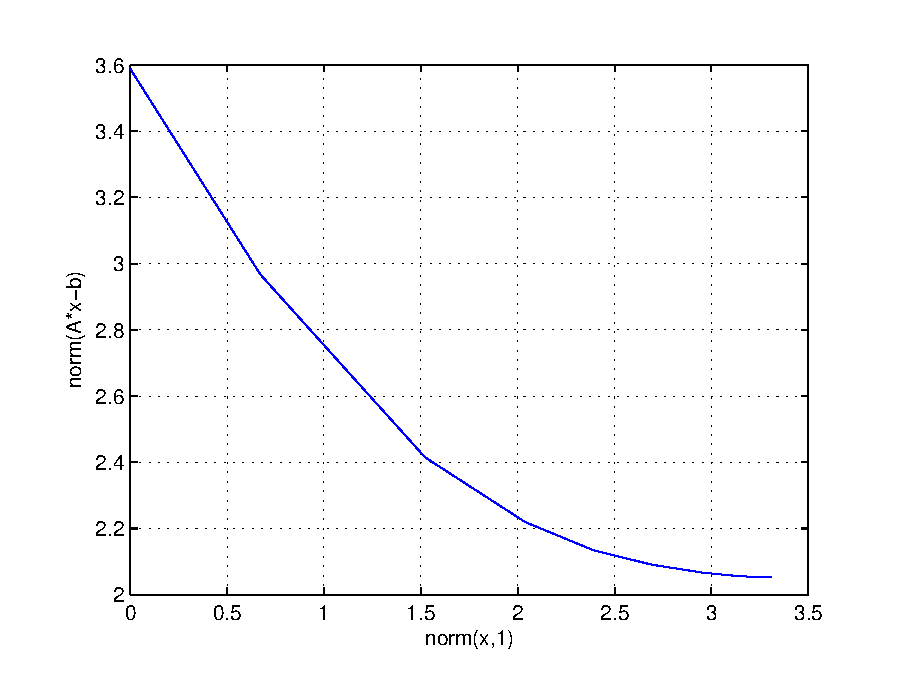
\includegraphics[width=4.5in]{tradeoff.eps}
\end{center}
~\\[-48pt]
\caption{An example trade-off curve from the \texttt{quickstart} demo, lines \ref{code:tradeoffbeg}-\ref{code:tradeoffend}.}
\label{fig:tradeoff}
\end{figure}

Line~\ref{code:tradeoff} of this code segment illustrates one of the
construction rules to be discussed in \S\ref{sec:rules} below. 
A basic principle of convex analysis is that a convex function
can be multiplied by a nonnegative scalar,
or added to another convex function, and the result
is then convex. 
\cvx recognizes such combinations and allows
them to be used anywhere a simple convex function can be---such as 
an objective function to be minimized, or on the appropriate side 
of an inequality constraint. So in our example, the expression
\begin{code}
	norm(A*x-b)+gamma(k)*norm(x,1)
\end{code}
on line~\ref{code:tradeoff}
is recognized as convex by \cvx, as long as \verb@gamma(k)@
is positive or zero. If \verb@gamma(k)@ were negative, then
this expression becomes the sum of a convex term and a concave
term, which causes \cvx
to generate the following error:
\index{constraint!nonconvex}
\begin{code}
??? Error using ==> cvx.plus
Disciplined convex programming error:
Addition of convex and concave terms is forbidden.
\end{code}

\newpage
\section{The basics}

\subsection{Data types for variables}
\index{variable!declaring}
\index{variable@\texttt{variable}}
\index{variables@\texttt{variables}}

As mentioned above, all variables must be declared using the \verb@variable@
command (or the \verb@variables@ command; see below) before they can be
used in constraints or an objective function. 

\index{variable!structure}
\index{variable!array}
\index{array variable}
\index{variable!complex}
\index{complex variable}
\index{variable!banded matrix}
\index{banded matrix variable}
\index{symmetric matrix variable}
\index{variable!symmetric matrix}
\index{diagonal matrix variable}
\index{variable!diagonal matrix}
\index{Hermitian matrix variable}
\index{variable!Hermitian matrix}
\index{Toeplitz matrix variable}
\index{variable!Toeplitz matrix}
Variables can be real or complex; and scalar, vector,
matrix, or $n$-dimensional arrays. In addition, matrices can have \emph{structure}
as well, such as symmetry or bandedness. The structure of a variable
is given by supplying a list of descriptive keywords after the name
and size of the variable.
For example, the code segment
\begin{code}
	variable w(50) complex;
	variable X(20,10);
	variable Y(50,50) symmetric;
	variable Z(100,100) hermitian toeplitz;
\end{code}
(inside a \cvx specification) declares that \verb@w@ is a complex
$50$-element vector variable, \verb@X@ is
a real $20 \times 10$ matrix variable, \verb@Y@ is
a real $50 \times 50$ symmetric matrix variable,
and \verb@Z@ is a complex $100 \times 100$ Hermitian Toeplitz 
matrix variable.
The structure keywords can be applied to
$n$-dimensional arrays as well:
each 2-dimensional ``slice'' of the array
is given the stated structure.  The currently supported structure
keywords are:
\begin{center}
\verb@banded(lb,ub)@\ \ \ \verb@complex@\ \ \ \verb@diagonal@\ \ \ \verb@hankel@\ \ \ \verb@hermitian@\ \ \ 
\verb@lower_bidiagonal@\ \ \ \verb@lower_hessenberg@\ \ \ \verb@lower_triangular@\ \ \ \verb@scaled_identity@\ \ \ 
\verb@skew_symmetric@\ \ \ \verb@symmetric@\ \ \ \verb@toeplitz@\ \ \ \verb@tridiagonal@\ \ \ 
\verb@upper_bidiagonal@\ \ \ \verb@upper_hankel@\ \ \ \verb@upper_hessenberg@\ \ \ \verb@upper_triangular@\ \ \ 
\end{center}
With a couple of exceptions, the structure keywords are self-explanatory:
\begin{itemize}
\item \verb@banded(lb,ub)@: the matrix is banded with a lower bandwidth \verb@lb@
and an upper bandwidth \verb@ub@. If both \verb@lb@ and \verb@ub@ are zero, then a 
diagonal matrix results. \verb@ub@ can be omitted, in which case it is set equal to \verb@lb@.
For example, \verb@banded(1,1)@ (or \verb@banded(1)@) is a tridiagonal matrix.
\item \verb@scaled_identity@: the matrix is a (variable) multiple of 
the identity matrix.
This is the same as declaring it to be diagonal and Toeplitz.
\item \verb@upper_hankel@: The matrix is Hankel (\ie, constant along antidiagonals), and zero
below the central antidiagonal, \ie, for $i+j>n+1$.
\end{itemize}
When multiple keywords are supplied, the resulting matrix structure is
determined by intersection; if the keywords conflict, then an error will result.

\index{variables@\texttt{variables}}
A \verb@variable@ statement can be used to declare only a single
variable, which can be a bit inconvenient if you have a lot of variables
to declare. For this reason, the \verb@variables@ statement
is provided which allows you to declare multiple variables; \ie,
\begin{code}
	variables x1 x2 x3 y1(10) y2(10,10,10);
\end{code}
The one limitation of the \verb@variables@ command is that it cannot
declare complex or structured arrays (\eg, \verb@symmetric@,
\emph{etc.}). These must be declared
one at a time, using the singular \verb@variable@ command.

\subsection{Objective functions}
\index{objective function}
\index{minimize@\texttt{minimize}}
\index{maximize@\texttt{maximize}}

Declaring an objective function requires
the use of the \verb@minimize@ or \verb@maximize@ function, as
appropriate.  The objective function in a call to \verb@minimize@ 
must be convex; the objective function in a call to \verb@maximize@
must be concave. At most one objective function may be declared in a 
given \cvx specification, and the objective function must have a
scalar value. (For the only exception to this rule, see the 
section on defining new functions in \S\ref{s-new-fcts}).

\index{feasibility}
\index{problem!feasibility}
\index{cvx_optval@\texttt{cvx\_optval}}
If no objective function is specified, the problem is interpreted
as a feasibility problem, which is the same as performing a minimization
with the objective function set to zero. In this case, \verb@cvx_optval@
is either \verb@0@, if a feasible point is found, or
\verb@+Inf@, if the constraints are not feasible.

\subsection{Constraints}
\index{constraint}
\index{constraint!equality}
\index{constraint!inequality}
\index{inequality!constraint}
\index{constraint!bounds}

The following constraint types are supported in \cvx:
\begin{itemize}
\item Equality \verb@==@ constraints, where both the left- and right-hand
sides are affine functions of the optimization variables.
\item Less-than \verb@<=@, \verb@<@ inequality constraints, where the left-hand
expression is convex, and the right-hand expression is concave.
\item Greater-than \verb@>=@, \verb@>@ constraints, where the left-hand
expression is concave, and the right-hand expression is convex.
\end{itemize}
In \cvx, the strict inequalities \verb@<@ and \verb@>@ are accepted,
but interpreted as the associated nonstrict inequalities, \verb@<=@
and \verb@>=@, respectively.   We encourage you to
use the nonstrict forms \verb@<=@ and \verb@>=@, since they are
mathematically correct.
(Future versions of \cvx might assign a slightly different meaning
to strict inequalities.)

These equality and inequality operators work for arrays.
When both sides of the constraint are arrays of the same size,
the constraint is imposed elementwise. For example, if \verb@a@ and \verb@b@
are $m \times n$ matrices, then \verb@a<=b@
is interpreted by \cvx as $mn$ (scalar) inequalities, \ie,
each entry of \verb@a@ must be less than or equal to
the corresponding entry of \verb@b@.
\cvx also handles cases where one side is 
a scalar and the other is an array.  This is interpreted as a
constraint for each element of the array, with the (same) scalar
appearing on the other side.
As an example, if \verb@a@ is an $m\times n$ matrix, then \verb@a>=0@ 
is interpreted as $mn$ inequalities: each element of the matrix
must be nonnegative.

Note also the important distinction between \verb@=@, which is an 
assignment, and \verb@==@, which imposes an equality constraint
(inside a \cvx specification); for more on this distinction,
see \S\ref{sec:eqass}.
Also note that the non-equality operator \verb@~=@ may \emph{not}
be used in a constraint; in any case, such constraints are 
rarely convex.
Inequalities cannot be used if either side is complex.

\cvx also supports a \emph{set membership} constraint; 
see \S\ref{sec:sets}.

\subsection{Functions}
\index{function}

The base \cvx function library
includes a variety of convex, concave, and affine functions
which accept \cvx variables or expressions as arguments.
Many are common Matlab functions
such as \verb@sum@, \verb@trace@, \verb@diag@, \verb@sqrt@,
\verb@max@, and \verb@min@,
re-implemented as needed to support \cvx; others are new
functions not found in Matlab.
A complete list of the functions in the base library 
can be found in \S\ref{s-functions}.
It's also possible to add your own new functions;
see \S\ref{s-new-fcts}.

An example of a function in the base library is
\verb@quad_over_lin@, which represents the
quadratic-over-linear function, defined as $f(x,y)=x^Tx/y$,
with domain $\R^n \times \R_{++}$, \ie,
$x$ is an arbitrary vector in $\R^n$, and $y$ is a positive
scalar.  (The function also accepts
complex $x$, but we'll consider real $x$ to keep things simple.)
The quadratic-over-linear function is convex in 
$x$ and $y$, and so can be 
used as an objective, in an appropriate constraint, or in a 
more complicated expression.
We can, for example, minimize the quadratic-over-linear
function of $(Ax-b,c^Tx+d)$ using
\begin{code}
	minimize( quad_over_lin( A*x-b, c'*x+d ) );
\end{code}
inside a \cvx specification,
assuming \verb@x@ is a vector optimization variable,
\verb@A@ is a matrix, \verb@b@
and \verb@c@ are vectors, and \verb@d@ is a scalar.
\cvx recognizes this objective expression as a convex 
function, since it is
the composition of a convex function (the quadratic-over-linear
function) with an affine function.

You can also use the function \verb@quad_over_lin@ \emph{outside}
a \cvx specification.   In this case, it just computes its (numerical)
value, given (numerical) arguments.
It's not quite the same as the expression 
\verb@((A*x-b)'*(A*x-b))/(c'*x+d)@,
however.  This expression makes sense, and returns a real number, 
when $c^Tx+d$ is negative; but \verb@quad_over_lin(A*x-b,c'*x+d)@
returns \verb@+Inf@ if $c^Tx+d \not > 0$.

\subsection{Sets}
\label{sec:sets}
\index{set}
\index{constraint!set}

\cvx supports the definition and use of convex sets.
The base library includes the cone of 
positive semidefinite $n \times n$ matrices,
the second-order or Lorentz cone, and various norm balls.
A complete list of sets supplied in the base library is given in 
\S\ref{s-functions}.

Unfortunately, the Matlab language does not have a 
set membership operator, such as \verb@x in S@, to denote $x \in S$.  
So in \cvx, we use a slightly different syntax to require
that an expression is in a set.
To represent a set we use a \emph{function} that returns
an unnamed variable that is required to be in the set.
Consider, for example, $\symm^n_+$, the cone of 
symmetric positive semidefinite $n \times n$ matrices.
In \cvx, we represent this by the function \verb@semidefinite(n)@,
which returns an unnamed new variable, that is constrained to be
positive semidefinite.
To require that the matrix expression \verb@X@ 
be symmetric positive semidefinite, we use the syntax \verb@X == semidefinite(n)@.
The literal meaning of this is that \verb@X@ is constrained to be 
equal to some unnamed variable, which is required to be 
an $n \times n$ symmetric positive semidefinite matrix. 
This is, of course, equivalent to saying that \verb@X@ must be
symmetric positive semidefinite.

\index{linear!matrix inequality|see{LMI}}
\index{semidefinite@\texttt{semidefinite}}
\index{SDP}
As an example, consider the constraint
that a (matrix) variable \verb@X@ is a correlation
matrix, \ie, it is symmetric, has unit diagonal elements, and 
is positive semidefinite.  In \cvx we can declare such a variable
and impose such constraints using
\begin{code}
	variable X(n,n) symmetric;
	X == semidefinite(n);
	diag(X) == ones(n,1);
\end{code}
The second line here imposes the constraint that \verb@X@
be positive semidefinite.
(You can read `\verb@==@' here as `is', so the second line can be 
read as `\verb@X@ is positive semidefinite'.)
The lefthand side of the third line
is a vector containing the diagonal elements of \verb@X@, whose 
elements we require to be equal to one. Incidentally, \cvx
allows us to simplify the third line to
\begin{code}
	diag(X) == 1;
\end{code}
because \cvx follows the Matlab convention of handling array/scalar
comparisons by comparing each element of the array independently with the scalar.

Sets can be combined in affine expressions, and we can constrain
an affine expression to be in a convex set.
For example, we can impose constraints of the form
\begin{code}
	A*X*A'-X == B*semidefinite(n)*B';
\end{code}
where \verb@X@ is an $n \times n$ symmetric variable matrix,
and \verb@A@ and \verb@B@ are $n \times n$  constant matrices.
This constraint requires that $AXA^T-X=BYB^T$, 
for some $Y \in \symm^n_+$.

\index{second-order cone}
\index{Lorentz cone|see{second-order cone}}
\index{SOCP}
\cvx also supports sets whose elements are ordered
lists of quantities.  As an example, consider the second-order or 
Lorentz cone,
\begin{equation}
	\lorentz^m = \Condset{ (x,y) \in \R^m\times\R }{ \| x \|_2 \leq y } = \epi \|\cdot\|_2,
\end{equation}
where $\epi$ denotes the epigraph of a function.
An element of $\lorentz^m$ is an ordered list, with two elements:
the first is an $m$-vector, and the second is a scalar.
We can use this cone to express the simple least-squares problem 
from \S\ref{sec:leastsquares} (in a fairly complicated way)
as follows:
\begin{equation}
	\begin{array}{ll}
		\text{minimize}   & y \\
		\text{subject to} & ( A x - b, y ) \in \lorentz^m.
	\end{array}
\end{equation}
\cvx uses Matlab's cell array facility to mimic this notation:
\begin{code}
	cvx_begin
	    variables x(n) y;
	    minimize( y );
	    subject to
	        { A*x-b, y } == lorentz(m);
	cvx_end
\end{code}
The function call \verb@lorentz(m)@ returns
an unnamed variable (\ie, a pair consisting of a vector and a 
scalar variable),
constrained to lie in the Lorentz cone of length \verb@m@. 
So the constraint in this
specification requires that the pair \verb@{ A*x-b, y }@
lies in the appropriately-sized Lorentz cone.

\subsection{Dual variables}
\index{dual variable}
\index{problem!dual}
\index{Lagrange multipler}

When a disciplined convex program is solved, the associated 
\emph{dual problem} is also solved.
(In this context, the original problem is called the \emph{primal
problem}.)
The optimal dual variables, each of which is associated with a 
constraint in the original problem,
give valuable information about the original problem,
such as the sensitivities with respect to perturbing the constraints
\cite[Ch.5]{BV:04}.
To get access to the optimal dual variables in \cvx, you 
simply declare them, and associate them with the constraints.
Consider, for example, the LP
\[
\begin{array}{llcll}
\mbox{minimize} & c^Tx \\
\mbox{subject to} & Ax \preceq b,
\end{array}
\]
with variable $x\in\Rn$, and $m$ inequality constraints.
The dual of this problem is
\[
\begin{array}{llcll}
\mbox{maximize} & - b^T y \\
\mbox{subject to} & c + A^T y = 0 \\ & y \succeq 0,
\end{array}
\]
where the dual variable $y$ is associated with the inequality
constraint $Ax\preceq b$ in the original LP.
To represent the primal problem and 
this dual variable in \cvx, we use the following syntax:
\begin{code}
	n = size(A,2);
	cvx_begin
	    variable x(n);
	    dual variable y;
	    minimize( c' * x );
	    subject to
	        y : A * x <= b;
	cvx_end
\end{code}	
The line 
\begin{code}
	dual variable y
\end{code}
tells \cvx that \verb@y@ will represent the dual variable, and the line
\begin{code}
	y : A * x <= b;
\end{code}
associates it with the inequality constraint. Notice how the
colon \verb@:@ operator is being used in a different manner than 
in standard Matlab, where it is used to construct numeric sequences
like \verb@1:10@.  This new behavior is in effect only
when a dual variable is present, so there should be no confusion 
or conflict. 
No dimensions are given
for \verb@y@; they are automatically determined from the constraint
with which it is associated. 
For example, if $m=20$, typing \verb@y@ at
the Matlab command prompt immediately before \verb@cvx_end@ yields
\begin{code}
y =
    cvx dual variable (20x1 vector)
\end{code}
It is not necessary to place the dual variable on the left side of the
constraint; for example, the line above can also be written in this way:
\begin{code}
	A * x <= b : y;
\end{code}
In addition, dual variables for inequality constraints
will always be nonnegative, which means that the sense of the inequality 
can be reversed without changing the dual variable's value; \ie,
\begin{code}
	b >= A * x : y;
\end{code}
yields an identical result. For \emph{equality} constraints, on the other
hand, swapping the left- and right- hand sides of an equality constraint
will \emph{negate} the optimal value of the dual variable.

After the \verb@cvx_end@ statement is processed, and assuming the
optimization was successful, \cvx assigns numerical values to
\verb@x@ and \verb@y@---the optimal primal and dual variable values,
respectively. Optimal primal and dual variables for this LP must
satisfy the \emph{complementary slackness conditions}
\begin{equation}
	y_i ( b - A x )_i = 0, \quad i=1,\dots,m.
\end{equation}
You can check this in Matlab with the line
\begin{code}
	y .* (b-A*x)
\end{code}
which prints out the products of the entries of \verb@y@ and 
\verb@b-A*x@, which should be nearly zero.
This line must be executed \emph{after} the \verb@cvx_end@ command
(which assigns numerical values to \verb@x@ and \verb@y@); it will
generate an error if it is executed inside the \cvx specification,
where \verb@y@ and \verb@b-A*x@ are still just abstract expressions.

\index{problem!infeasible}
\index{infeasible problem}
If the optimization is \emph{not} successful, because either the problem
is infeasible or unbounded, then \verb@x@ and \verb@y@ will have different
values. In the unbounded case, \verb@x@ will contain an \emph{unbounded direction};
\ie, a point $x$ satisfying
\begin{equation}
	c^T x = -1, \quad A x \preceq 0,
\end{equation}
and \verb@y@ will be filled with \verb@NaN@ values, reflecting the fact
that the dual problem is infeasible. In the infeasible case,
\verb@x@ is filled with \verb@NaN@ values, while \verb@y@
contains an \emph{unbounded dual direction}; \ie, a point $y$ satisfying
\begin{equation}
	b^T y = -1, \quad A^T y = 0, \quad y \succeq 0
\end{equation}
Of course, the precise interpretation of primal and dual points and/or
directions depends on the structure of the problem. See references
such as \cite{BV:04} for more on the interpretation of dual information.

\cvx also supports the declaration of \emph{indexed} dual
variables. These prove useful when the \emph{number} of constraints in
a model (and, therefore, the number of dual variables) depends upon the
parameters themselves. For more information on indexed dual variables,
see \S\ref{sec:indexeddual}.

\subsection{Expression holders}
\label{sec:holders}
\index{expression holder}
\index{expression@\texttt{expression}}
\index{expressions@\texttt{expressions}}

Sometimes it is useful to store a \cvx expression into a Matlab variable for
future use. For instance, consider the following \cvx script:
\begin{code}
	variables x y
	z = 2 * x - y;
	square( z ) <= 3;
	quad_over_lin( x, z ) <= 1;
\end{code}
The construction \verb@z = 2 * x - y@ is \emph{not} an equality constraint; it
is an assignment. It is storing an intermediate calculation \verb@2 * x - y@,
which is an affine expression,
which is then used later in two different constraints. We call \verb@z@ an
\emph{expression holder} to differentiate it from a 
formally declared \verb@cvx@ variable. For more on the critical
differences between assignment and equality, see Section \S\ref{sec:eqass}.

Often it will be useful to accumulate an array of expressions into a single
Matlab variable. 
Unfortunately, a somewhat technical detail of the Matlab object
model can cause problems in such cases. Consider this construction:
\begin{code}
variable u(9);
x(1) = 1;
for k = 1 : 9,
    x(k+1) = sqrt( x(k) + u(k) );
end
\end{code}
This seems reasonable enough: \verb@x@ should be a vector whose first value is
\verb@1@, and whose subsequent values are concave \cvx expressions. 
But if you try this in a \cvx model, Matlab will give you a rather 
cryptic error:
\begin{code}
??? The following error occurred converting from cvx to double:
Error using ==> double
Conversion to double from cvx is not possible.
\end{code}
The reason this occurs is that the Matlab variable \verb@x@ is initialized as
a numeric array when the assignment \verb@x(1)=1@ is made;
and Matlab will not permit \cvx objects to be subsequently inserted into 
numeric arrays. 

The solution is to explicitly \emph{declare} \verb@x@ to be an 
expression holder before assigning values to it. 
We have provided keywords \verb@expression@
and \verb@expressions@ for just this purpose, for declaring a single or 
multiple expression holders for future assignment. Once an expression holder
has been declared, you may freely insert both numeric and \cvx expressions
into it. For example, the previous
example can be corrected as follows:
\begin{code}
variable u(9);
expression x(10);
x(1) = 1;
for k = 1 : 9,
    x(k+1) = sqrt( x(k) + u(k) );
end
\end{code}
\cvx will accept this construction without error.
You can then use the concave expressions \verb@x(1)@, \ldots, \verb@x(10)@
in any appropriate ways; for example, you could maximize \verb@x(10)@.

The differences between a \verb@variable@ object and an \verb@expression@ object
are quite significant. 
A \verb@variable@ object holds an optimization
variable, and cannot be overwritten or assigned in the \cvx specification.
(After solving the problem, however, \cvx will overwrite 
optimization variables with optimal values.) 
An \verb@expression@ object, on the other hand, is initialized to zero, 
and should be thought of as a temporary place to store \cvx expressions;
it can be assigned to, freely re-assigned, and overwritten in a \cvx
specification.

Of course, as our first example
shows, it is not always \emph{necessary} to declare an expression holder before
it is created or used. But doing so provides an extra measure
of clarity to models, so we strongly recommend it.

\newpage
\section{The DCP ruleset}
\label{sec:rules}
\index{DCP!ruleset}

\cvx enforces the conventions dictated by the
disciplined convex programming ruleset, or \emph{DCP ruleset} for short.
\cvx will issue an error message whenever it encounters a violation 
of any of the rules, so it is important to understand
them before beginning to build models. 
The rules are drawn from basic principles of convex analysis, and 
are easy to learn, once you've had an exposure to convex analysis
and convex optimization.

The DCP ruleset is a set of sufficient, but not necessary, conditions
for convexity.  So it is possible to construct expressions that violate
the ruleset but are in fact convex. 
As an example consider the entropy function,
$-\sum_{i=1}^n  x_i \log x_i$,
defined for $x>0$, which is concave.
If it is expressed as
\begin{code}
	- sum( x .* log( x ) )
\end{code}
\cvx will reject it, because its concavity does not 
follow from any of the composition rules.
(Specifically, it violates the 
no-product rule described in \S\ref{sec:noproduct}.)
Problems involving entropy, however, can be solved, by explicitly
using the entropy function, 
\begin{code}
	sum(entr( x ))
\end{code}
which is in the base \cvx library, and thus recognized as 
concave by \cvx.
If a convex (or concave) function is not recognized as
convex or concave by \cvx, it can be added as a new atom;
see \S\ref{s-new-fcts}.

As another example consider the function $\sqrt{x^2+1}=\|[x~1]\|_2$,
which is convex.
If it is written as
\begin{code}
	norm([x 1])
\end{code}
(assuming \verb@x@ is a scalar variable or affine expression)
it will be recognized by \cvx as a convex expression, and therefore 
can be used in (appropriate) constraints and objectives.
But if it is written as
\begin{code}
	sqrt(x^2+1)
\end{code}
\cvx will reject it, since convexity of this function does not follow
from the \cvx ruleset.

%If a convex (or concave) function is not recognized as
%convex or concave by \cvx, it can be added as a new atom;
%see \S\ref{s-new-fcts}.

%At first, these restrictions may seem inconvenient,
%especially to those accustomed to the more permissive nature of 
%more traditional modeling frameworks.
%We hope you will find that the rules are, in fact, not 
%particularly restrictive
%in practice; and certainly that they are a small price to pay 
%for the considerable benefits they allow: automatic convexity 
%verification, automatic
%conversion to solvable form, and full support for nonsmooth functions. 

%The rules for constructing geometric programs are not covered in this
%section. To simplify the discussion, those rules will be introduced
%later in \S\ref{sec:geometric}. The remainder
%of this section applies specifically to traditional
%convex programs with no geometric variables, objectives, or constraints.

\subsection{A taxonomy of curvature}
\label{sec:taxonomy}

In disciplined convex programming, a scalar expression is classified
by its \emph{curvature}. There are four
categories of curvature:
\emph{constant}, \emph{affine}, \emph{convex}, and \emph{concave}.
For a function $f:\Rn\rightarrow\R$ defined on all $\Rn$,
the categories have the following meanings:
\begin{equation*}
\begin{array}{lc@{\,}lc}
\text{constant:}    & f(\alpha x + (1-\alpha)y) & = f(x) &
 \forall x,y\in\Rn,~\alpha\in\R\\
\text{affine:}      & f(\alpha x + (1-\alpha)y) & =
 \alpha f(x) + (1-\alpha) f(y) & \forall x,y\in\Rn,~\alpha\in\R \\
\text{convex:}  & f(\alpha x + (1-\alpha)y)
 & \leq \alpha f(x) + (1-\alpha) f(y) & \forall x,y\in\Rn,~\alpha\in [0,1] \\
\text{concave:}     \quad & f(\alpha x + (1-\alpha)y) & 
\geq \alpha f(x) + (1-\alpha) f(y) &
\forall x,y\in\Rn,~\alpha\in [0,1] 
\end{array}
\end{equation*}
Of course, there is significant
overlap in these categories. 
For example, constant expressions are also affine,
and (real) affine expressions are both convex and concave.

Convex and concave expressions are real by definition. Complex constant
and affine expressions can be constructed, but their usage is more limited;
for example, they cannot appear as the left- or right-hand side of an inequality
constraint.

\subsection{Top-level rules}
\label{sec:toplevel}

\index{feasibility}
\index{problem!feasibility}
\cvx supports three different types of disciplined convex programs:
\begin{itemize}
\item A \emph{minimization problem}, consisting of a convex objective function
and zero or more constraints.
\item A \emph{maximization problem}, consisting of a concave objective function
and zero or more constraints.
\item A \emph{feasibility problem}, consisting of one or more constraints.
\end{itemize}
%The validity of each constraint is determined \emph{individually}, so it is not
%sufficient for the intersection of the constraints to be convex. For example, the set
%\begin{equation*}
	%\Condset{ x\in \R }{ x^2 \geq 1, ~ x \geq 0 }
%\end{equation*}
%is convex (it is just the interval $[1,\infty)$), but its description
%includes a nonconvex constraint $x^2 \geq 1$.

\subsection{Constraints}

Three types of constraints may be specified in disciplined convex programs:
\begin{itemize}
\item An \emph{equality constraint}, constructed using \verb@==@,
where both sides are affine.
\item A \emph{less-than inequality constraint}, using either
\verb@<=@ or \verb@<@,
where the left side is convex and the right side is concave.
\item A \emph{greater-than inequality constraint}, using either
\verb@>=@ or \verb@>@,
where the left side is concave and the right side is convex.
\end{itemize}
\emph{Non}-equality constraints, constructed using
\verb@~=@, are never allowed.   (Such constraints are not convex.)

One or both sides of an equality constraint may be complex; inequality constraints,
on the other hand, must be real. A complex equality
constraint is equivalent to two real equality constraints, one for the real part
and one for the imaginary part. 
An equality constraint with
a real side and a complex side has the effect of constraining the 
imaginary part of the complex side to be zero.

As discussed in \S\ref{sec:sets} above, \cvx enforces set 
membership constraints (\eg, $x\in S$) using
equality constraints. 
The rule that both sides of an equality constraint
must be affine  applies to set membership constraints as well. 
In fact, the returned value of set atoms like 
\verb@semidefinite()@ and \verb@lorentz()@ is affine,
so it is sufficient to simply verify the remaining portion
of the set membership constraint. For composite values like
\verb@{ x, y }@, each element must be affine.

In this version, 
strict inequalities \verb@<@, \verb@>@ are interpreted
identically to nonstrict inequalities \verb@>=@, \verb@<=@. 
Eventually \cvx will flag strict inequalities so that they 
can be verified after the optimization is carried out.

\subsection{Expression rules}
\label{sec:noproduct}

So far, the rules as stated are not particularly restrictive, 
in that all convex programs (disciplined or otherwise) 
typically adhere to them.
What distinguishes disciplined convex programming from more general
convex programming are the rules governing
the construction of the expressions used in objective functions and
constraints.

Disciplined convex programming determines the curvature of scalar
expressions by recursively applying the following rules.
While this list may seem long, it is for the most part an enumeration of basic
rules of convex analysis for combining convex, concave, and affine forms: sums,
multiplication by scalars, and so forth.
\begin{itemize}
\item A valid constant expression is
\begin{itemize}
\item any well-formed Matlab expression that 
evaluates to a finite value.
\end{itemize}
\item A valid affine expression is
\begin{itemize}
\item a valid constant expression;
\item a declared variable;
\item a valid call to a function in the atom library with an affine result;
\item the sum or difference of affine expressions;
\item the product of an affine expression and a constant.
\end{itemize}
\item A valid convex expression is
\begin{itemize}
\item a valid constant or affine expression;
% , or log-convex expression (\S\ref{sec:gpmode});
\item a valid call to a function in the atom library with a convex result;
\item an affine scalar raised to a constant power $p\geq 1$, $p\neq 3,5,7,9,...$;
\item a convex scalar quadratic form (\S\ref{sec:quadforms});
\item the sum of two or more convex expressions;
\item the difference between a convex expression and a concave expression;
\item the product of a convex expression and a nonnegative constant;
\item the product of a concave expression and a nonpositive constant;
\item the negation of a concave expression.
\end{itemize}
\item A valid concave expression is
\begin{itemize}
\item a valid constant or affine expression;
\item a valid call to a function in the atom library with a concave result;
\item a concave scalar raised to a power $p\in(0,1)$;
\item a concave scalar quadratic form (\S\ref{sec:quadforms});
\item the sum of two or more concave expressions;
\item the difference between a concave expression and a convex expression;
\item the product of a concave expression and a nonnegative constant; 
\item the product of a convex expression and a nonpositive constant;
\item the negation of a convex expression.
\end{itemize}
\end{itemize}
If an expression cannot be categorized by this ruleset,
%(or their geometric programming counterparts described 
%in \S\ref{sec:gp-expressions}), 
it is rejected by \cvx.
For matrix and array expressions, these rules
are applied on an elementwise basis.
We note that the set of rules listed above is redundant;
there are much smaller, equivalent sets of rules.

Of particular note is that these expression rules generally 
forbid \emph{products}
between nonconstant expressions,  
with the exception of scalar quadratic forms 
(see \S\ref{sec:quadforms} below). 
For example, the expression \verb@x*sqrt(x)@ happens to be a 
convex function of \verb@x@, but its convexity cannot be verified
using the \cvx ruleset, and so is rejected.
(It can be expressed as \verb@x^(3/2)@ or \verb@pow_p(x,3/2)@, however.)
We call this the \emph{no-product rule},
and paying close attention to it will go a long way to insuring that the
expressions you construct are valid.

%The function $\sqrt{x^2+1}$, written as the expression 
%\verb@sqrt(x^2+1)@, is another example of a convex 
%function that cannot be verified 
%as convex using the \cvx ruleset.
%(It is recognized as convex when it is written as \verb@norm([x 1])@,
%since \verb@norm@ is in the \cvx base library of convex functions,
%and \verb@[x 1]@ is recognized as an affine expression.)

\subsection{Functions}
\label{sec:functions}

%Because functions in the \cvx atom library are created in the 
%Matlab language,
%they differ in certain ways from functions described in a 
%formal mathematical sense,
%so we address these differences here.  
%We continue
%to set aside geometric programming for now, and
%consider only the traditional convex programming case.

\index{convex!function}
\index{concave!function}
\index{function!concave}
\index{function!convex}
\index{nonincreasing}
\index{nondecreasing}
\index{monotonicity}
\index{function!monotonicity}
\index{function!affine}
\index{affine function}
In \cvx, functions are categorized in two attributes: \emph{curvature}
(\emph{constant}, \emph{affine},
\emph{convex}, or \emph{concave}) and
\emph{monotonicity}
(\emph{nondecreasing}, \emph{nonincreasing}, or \emph{nonmonotonic}).
Curvature determines the conditions
under which they can appear in expressions according to the
expression rules given in \S\ref{sec:noproduct} above.
Monotonicity determines
how they can be used in function  compositions, 
as we shall see in \S\ref{sec:compositions} below.

For functions with only one argument, the categorization is 
straightforward.  Some examples are given in the table below.
\begin{center}
\begin{tabular}{llll}
Function & Meaning & Curvature & Monotonicity \\ \hline
	\verb@sum( x )@ & $\sum_i x_i$ & affine & nondecreasing \\
	\verb@abs( x )@ & $|x|$ & convex & nonmonotonic \\
	%\verb@log( x )@ & $\log x$ & concave, nondecreasing
	\verb@sqrt( x )@ & $\sqrt x$ & concave & nondecreasing
\end{tabular}
\end{center}

Following standard practice in convex analysis, convex functions
are interpreted as $+\infty$ when the argument is outside the domain
of the function, and concave functions are interpreted as $-\infty$
when the argument is outside its domain.
In other words, convex and concave functions in \cvx are interpreted
as their \emph{extended-valued extensions}.

This has the effect of automatically constraining the argument of 
a function to be in the function's domain.
For example, if we form \verb@sqrt(x+1)@ in a \cvx specification,
where \verb@x@ is a variable, then
\verb@x@ will automatically be constrained to be larger than or
equal to $-1$.  There is no need to add a separate constraint,
\verb@x>=-1@, to enforce this.

Monotonicity of a function is determined in the extended sense,
\ie, \emph{including the values of the argument outside its domain}.
For example, \verb@sqrt(x)@ is determined to be nondecreasing since
its value is constant ($-\infty$) 
for negative values of its argument; then jumps \emph{up} to $0$ 
for argument zero, and increases for positive values of its 
argument.

\cvx does \emph{not} consider a function to be
convex or concave if it is so only over a portion of its domain,
even if the argument is constrained to lie in one of these portions.
As an example, consider the function $1/x$.
This function is convex for $x>0$, and concave for $x<0$.
But you can never write \verb@1/x@ in \cvx (unless \verb@x@ is constant),
even if you have imposed a constraint such as \verb@x>=1@, which restricts
\verb@x@ to lie in the convex portion of function $1/x$.
You can use the \cvx function \verb@inv_pos(x)@, defined as
$1/x$ for $x>0$ and $\infty$ otherwise, for the convex portion of
$1/x$; \cvx recognizes this function as convex and nonincreasing.
In \cvx, you can express the concave portion of $1/x$, 
where $x$ is negative, using \verb@-inv_pos(-x)@, which will be correctly
recognized as concave and nonincreasing.

For functions with multiple arguments,
curvature is always considered \emph{jointly}, but monotonicity
can be considered on an \emph{argument-by-argument} basis. For example,
\begin{center}
\begin{tabular}{lll}
	\verb@quad_over_lin( x, y )@ & $\Cases{|x|^2/y&y> 0\\+\infty&y\leq 0}$ & convex, nonincreasing in $y$
\end{tabular}
\end{center}
is jointly convex in both arguments, but it is monotonic 
only in its second argument.

In addition, some functions are convex, concave, or affine only for 
a \emph{subset} of its arguments. For example, the function
\begin{center}
\begin{tabular}{lll}
	\verb@norm( x, p )@ & $\|x\|_p~~(1 \leq p)$ & convex in $x$, nonmonotonic
\end{tabular}
\end{center}
is convex only in its first argument. Whenever this function is used
in a \cvx specification, then, the remaining
arguments must be constant, or \cvx will issue an error message. Such arguments
correspond to a function's parameters in mathematical terminology; \eg,
\begin{equation*}
	f_p(x):\R^n\rightarrow\R, \quad f_p(x) \triangleq \|x\|_p
\end{equation*}
So it seems fitting that we should refer to such arguments as \emph{parameters}
in this context as well. Henceforth, whenever we speak of a \cvx function
as being convex, concave, or affine, we will assume that its parameters are
known and have been given appropriate, constant values.

\subsection{Compositions}
\label{sec:compositions}
\index{composition}
\index{function!composition}

A basic rule of convex analysis is that convexity is closed under 
composition with an affine mapping. 
This is part of the DCP ruleset as well:
\begin{itemize}
\item A convex, concave, or affine function may accept an affine expression
(of compatible size) as an argument.
The result is convex, concave, or affine, respectively.
\end{itemize}
For example, consider the function \verb@square( x )@, which is provided
in the \cvx atom library. 
This function squares its argument; \ie, it computes
\verb@x.*x@. 
(For array arguments, it squares each element independently.)
It is in the \cvx atom library, and known to be convex, provided its
argument is real.  So if \verb@x@ is a real variable of dimension $n$,
\verb@a@ is a constant $n$-vector, and \verb@b@ is a constant,
the expression
\begin{code}
	square( a' * x + b )
\end{code}
is accepted by \cvx, which knows that it is convex.

The affine composition rule above is a special case of a more
sophisticated composition rule, which we describe now. 
We consider a function, of known curvature and monotonicity, that accepts
multiple arguments.  For \emph{convex} functions, the rules are:
\begin{itemize}
\item If the function is nondecreasing in an argument,
that argument must be convex.
\item If the function is nonincreasing in an argument,
that argument must be concave.
\item If the function is neither nondecreasing or nonincreasing
in an argument, that argument must be affine.
\end{itemize}
If each argument of the function satisfies these rules, then the expression
is accepted by \cvx, and is classified as convex.
Recall that a constant or affine expression is both convex and concave,
so any argument can be affine, including as a special case, constant. 

The corresponding rules for a concave function are as follows:
\begin{itemize}
\item If the function is nondecreasing in an argument,
that argument must be concave.
\item If the function is nonincreasing in an argument,
that argument must be convex.
\item If the function is neither nondecreasing or nonincreasing
in an argument, that argument must be affine.
\end{itemize}
In this case, the expression is accepted by \cvx, and classified
as concave.

For more background on these composition rules, see \cite[\S3.2.4]{BV:04}.
In fact, with the exception of scalar quadratic expressions,
the entire DCP ruleset can be thought of as special cases
of these six rules.

Let us examine some examples.
The maximum function is convex and nondecreasing in every argument,
so it can accept any convex expressions as arguments.
For example, if \verb@x@ is a vector variable, then 
\begin{code}
	max( abs( x ) )
\end{code}
obeys the first of the six composition rules and is therefore accepted
by \cvx, and classified as convex.
%In fact, the infinity-norm function \verb@norm( x, Inf )@
%is defined in exactly this manner. 


As another example, consider the sum function, which is both
convex and concave (since it is affine), and nondecreasing 
in each argument.  Therefore the expressions
\begin{code}
	sum( square( x ) )
	sum( sqrt( x ) )
\end{code}
are recognized as valid in \cvx, and classified as 
convex and concave, respectively.
The first one follows from the first rule for convex functions;
and the second one follows from the first rule for concave functions.

Most people who know basic convex analysis like to think of these
examples in terms of the more specific rules:
a maximum of convex functions is convex, and a sum of convex (concave)
functions is convex (concave). 
But these rules are just special cases of the general composition 
rules above.
Some other well known basic rules that follow from the 
general composition rules are:
a nonnegative multiple of a convex (concave) function is convex (concave);
a nonpositive multiple of a convex (concave) function is concave (convex).

Now we consider a more complex example in depth. Suppose
\verb@x@ is a vector variable, and
\verb@A@, \verb@b@, and \verb@f@ are 
constants with appropriate dimensions.  \cvx recognizes the
expression
\begin{code}
sqrt(f'*x) + min(4,1.3-norm(A*x-b))
\end{code}
as concave. Consider the term \verb@sqrt(f'*x)@. \cvx
recognizes that \verb@sqrt@ is concave and \verb@f'*x@ is affine,
so it concludes that \verb@sqrt(f'*x)@ is concave. Now consider
the second term \verb@min(4,1.3-norm(A*x-b))@. \cvx
recognizes that \verb@min@ is concave and nondecreasing, so
it can accept concave arguments.
\cvx recognizes that \verb@1.3-norm(A*x-b)@ is concave,
since it is the difference of a constant and a convex function. So \cvx
concludes that the second term is also concave.
The whole expression is then recognized as concave,
since it is the sum of two concave functions.

The composition rules are sufficient but not necessary for
the classification to be correct,
so some expressions which are in fact convex or concave will fail to
satisfy them, and so will be rejected by \cvx.
For example, if \verb@x@ is a vector variable, the
expression
\begin{code}
	sqrt( sum( square( x ) ) )
\end{code}
is rejected by \cvx, because there is no rule governing the composition
of a concave nondecreasing function with a convex function.
Of course, the workaround is simple in this case: use \verb@norm( x )@ instead,
since \verb@norm@ is in the atom library and known by \cvx to be convex.

\subsection{Monotonicity in nonlinear compositions}

Monotonicity is a critical aspect of the rules for nonlinear compositions. 
This has some consequences that are not so obvious, as we shall demonstrate here
by example. Consider the expression
\begin{code}
	square( square( x ) + 1 )
\end{code}
where \verb@x@ is a scalar variable.
This expression is in fact convex, since
$(x^2+1)^2 = x^4+2x^2+1$ is convex.
But \cvx will reject the expression, because the outer \verb@square@
cannot accept a convex argument.  Indeed, the square of a convex function
is not, in general, convex: for example, $(x^2-1)^2 = x^4-2x^2+1$ is
not convex.

There are several ways to modify the expression above to
comply with the ruleset.
One way is to write it as \verb@x^4 + 2*x^2 + 1@,
which \cvx recognizes as convex, since
\cvx allows positive even integer powers using the \verb@^@ operator.
(Note that the same technique, applied to the function $(x^2-1)^2$,
will fail, since its second term is concave.)
%But let us look at an alternative for further illustration.
%One is to recognize that a constraint such as
%\begin{code}
	%square( square( A * x + b ) ) <= 1
%\end{code}
%is equivalent to
%\begin{code}
	%square( A * x + b ) <= z
	%square( z ) <= 1
%\end{code}
%where \verb@z@ is a new variable of the same size as \verb@A*x+b@.
%The equivalence of this decomposition
%is a direct consequence of the monotonicity of 
%\verb@square@ when \verb@z@
%is nonnegative. In fact, \cvx performs this decomposition itself for
%those nonlinear compositions that it accepts; \ie, those that
%satisfy the DCP ruleset.

Another approach is to use the alternate outer function 
\verb@square_pos@,
included in the \cvx library, which represents the
function $(x_+)^2$, where $x_+ = \max\{0,x\}$.
Obviously, \verb@square@ and \verb@square_pos@ coincide when their
arguments are nonnegative. 
But \verb@square_pos@ is nondecreasing, so it
can accept a convex argument.
Thus, the expression
\begin{code}
	square_pos( square( x ) + 1 )
\end{code}
is mathematically equivalent to the rejected version above
(since the argument to the outer function is always positive),
but it satisfies the DCP ruleset and is therefore accepted by \cvx.

This is the reason several functions in the \cvx atom library come in two
forms: the ``natural'' form, and one that is modified in such a way 
that it is monotonic, and can therefore 
be used in compositions. Other such ``monotonic extensions''
include \verb@sum_square_pos@ and \verb@quad_pos_over_lin@. If you are
implementing a new function yourself, you might wish to consider if
a monotonic extension of that function would also be useful.

%By the way, if you're going to encounter the same function with several
%different arguments, you might want to define a new function, say,
%\verb@square_of_square_plus_one@,
%using any of the above techniques.
%(See \S\ref{s-new-fcts} for how to do this.)
%This allows us to write the original expression as
%\begin{code}
	%square_of_square_plus_one( x )
%\end{code}
%This new function \verb@square_of_square_plus_one@ can now be used 
%in any other expression, as long as its argument is affine.

\subsection{Scalar quadratic forms}
\label{sec:quadforms}

\index{function!quadratic}
\index{quadratic form}

In its original form described in \cite{Gra:04,GBY},
the DCP ruleset forbids even the use of simple
quadratic expressions such as \verb@x * x@ 
(assuming \verb@x@ is a scalar variable).
For practical reasons, we have chosen to make an exception to the ruleset to 
allow for the recognition of certain specific quadratic forms that map
directly to certain convex quadratic functions (or their concave negatives)
in the \cvx atom library:
\begin{center}
\begin{tabular}{lll}
\verb@conj( x ) .* x@ & is replaced with & \verb@square( x )@ \\
\verb@y' * y@ & is replaced with & \verb@sum_square( y )@\\
\verb@(A*x-b)'*Q*(Ax-b)@ & is replaced with &
\verb@quad_form( A * x - b, Q )@
\end{tabular}
\end{center}
\cvx detects the quadratic expressions
such as those on the left above, and determines whether or not they
are convex or concave; and if so, translates them to an equivalent
function call, such as those on the right above.

\cvx examines each \emph{single} product of affine expressions, and each
\emph{single} squaring of an affine expression, checking for 
convexity; it will not check, for example, sums of products of 
affine expressions.
For example, given scalar variables \verb@x@ and \verb@y@,
the expression
\begin{code}
	x ^ 2 + 2 * x * y + y ^2
\end{code}
will cause an error in \cvx, because the second of the three terms
\verb@2 * x * y@, is neither convex nor concave.
But the equivalent expressions
\begin{code}
	( x + y ) ^ 2
	( x + y ) * ( x + y )
\end{code}
will be accepted. \cvx actually completes the
square when it comes across a scalar quadratic form, so the form
need not be symmetric. For example,
if \verb@z@ is a vector variable, \verb@a@, \verb@b@ are constants,
and \verb@Q@ is positive definite, then
\begin{code}
	( z + a )' * Q * ( z + b )
\end{code}
will be recognized as convex. Once a quadratic form has been verified by \cvx,
it can be freely
used in any way that a normal convex or concave expression can be,
as described in \S\ref{sec:noproduct}.

Quadratic forms should actually be used less
frequently in disciplined convex programming
than in a more traditional mathematical programming framework,
where a quadratic form is often a smooth substitute 
for a nonsmooth form that one truly wishes to use. In
\cvx, such substitutions are rarely necessary, because of its support
for nonsmooth functions. For example,
the constraint
\begin{code}
	sum( ( A * x - b ) .^ 2 ) <= 1
\end{code}
is equivalently represented using the Euclidean norm:
\begin{code}
	norm( A * x - b ) <= 1
\end{code}
With modern solvers, the second form can be represented using a second-order cone
constraint---so the second form may actually be more efficient. So we encourage
you to re-evaluate the use of quadratic forms in your models, in light of the
new capabilities afforded by disciplined convex programming.


\newpage
\section{Adding new functions to the \cvx atom library}
\label{s-new-fcts}
\index{function!defining new}
\index{defining new function}

%The restrictions imposed by the DCP ruleset imply that,
%for a fixed atom library, the variety of constraints and objective 
%functions that can be constructed is limited. Thus in order to preserve 
%generality in disciplined convex programming, the atom library must be extensible;
\cvx allows new convex and concave functions to be defined and added to the
atom library, in two ways, described in this section.
The first method is simple, and can (and should) be used by 
many users of \cvx, since it requires only a knowledge of the 
basic DCP ruleset.
%Indeed, we have steadily added new functions to the library over
%time, based on our own needs and those of users who have given us feedback.
%So if you encounter a useful convex or concave function that is not supported
%by \cvx, we invite you to tell us about it. Please understand, however, that not
%every such function can be added, due to limitations in the solver.
%It is also possible for a \emph{user} of \cvx to define
%new convex and concave functions to be be used in \cvx specifications.
%This can be accomplished in two ways, both of
%which we describe in this section. 
The second method is very powerful, but a bit complicated, and
should be considered an advanced technique, to be attempted only by those 
who are truly comfortable
with convex analysis, disciplined convex programming,
and \cvx in its current state.

Please do let us know if you have implemented a convex or concave function
that you think would be useful to other users; we will be happy to 
incorporate it in a future release.

\subsection{New functions via the DCP ruleset}

The simplest way to construct a new function that works within \cvx
is to construct it using expressions that fully conform to the DCP
ruleset.
\index{deadzone function}
\index{function!deadzone}
To illustrate this, consider the convex \emph{deadzone} function,
defined as
\[
f(x) = \max \{ |x|-1, 0 \} =
\left\{ \begin{array}{ll}
0 & |x| \leq 1\\
x-1 & x > 1\\
-1-x & x <-1
\end{array}\right.
\]
To implement this function in \cvx, simply create a file \verb@deadzone.m@
containing
\begin{code}
	function y = deadzone( x )
	y = max( abs( x ) - 1, 0 )
\end{code}
This function works just as you expect it would outside of \cvx---\ie,
when its argument is numerical. But thanks to Matlab's operator
overloading capability, it will also work within \cvx if called with an affine
argument. \cvx will properly conclude that the function is convex,
because all of the operations
carried out conform to the rules of DCP:
\verb@abs@ is recognized as a convex function; we can subtract 
a constant from it, and we can take the maximum of the result and 
\verb@0@, which yields a convex function. So we are free
to use \verb@deadzone@ anywhere in a \cvx specification that we might
use \verb@abs@, for example,
because \cvx knows that it is a convex function.

Let us emphasize that when defining a function this way, the
expressions you use \emph{must} conform to the DCP ruleset, just as
they would if they had been inserted directly into a \cvx model. For
example, if we replace \verb@max@ with \verb@min@ above; \eg,
\begin{code}
	function y = deadzone_bad( x )
	y = min( abs( x ) - 1, 0 )
\end{code}
then the modified function fails to meet the DCP ruleset. The
function will work \emph{outside} of a \cvx specification,
happily computing
the value $\min \{|x|-1,0\}$ for a \emph{numerical}
argument $x$. But inside a \cvx specification, invoked 
with a nonconstant argument, it will not work, because
it doesn't follow the DCP composition rules.

\subsection{New functions via partially specified problems}

A more advanced method for defining new functions in \cvx
relies on the following basic result of convex analysis.
Suppose that $S\subset\R^n\times\R^m$ is a convex set and 
$g:(\R^n\times\R^m)\rightarrow(\R\cup+\infty)$ is a convex function. 
Then
\begin{equation}
	\label{eq:partial}
	f:\R^n\rightarrow(\R\cup+\infty), \quad 
f(x) \triangleq \inf\Condset{g(x,y)}{\exists y,~(x,y)\in S }
\end{equation}
is also a convex function. (This rule is sometimes called
the \emph{partial minimization rule}.)
We can think of the convex function $f$ as the optimal value of
a family of convex optimization problems, indexed or parametrized
by $x$,
\[
\begin{array}{ll}
\mbox{minimize} & g(x,y) \\
\mbox{subject to} & (x,y) \in S
\end{array}
\]
with optimization variable $y$.

One special case should be very familar: if $m=1$ and
$g(x,y)\triangleq y$, then
\[
	f(x) \triangleq \inf\Condset{y}{\exists y,~(x,y)\in S}
\]
gives the classic \emph{epigraph} representation of $f$:
\[
\epi f = S+ \left( \{ 0 \} \times \reals_+ \right),
\]
where $0 \in \reals^n$.
\index{function!epigraph}
\index{epigraph}

In \cvx you can define a convex
function in this very manner, that is, as the optimal value of a 
parameterized family of disciplined convex programs. 
We call the underlying convex program in such cases
an \emph{incomplete specification}---so named because
the parameters (that is, the function inputs)
are unknown when the specification is
constructed. The concept of incomplete 
specifications can at first seem a bit complicated,
but it is very powerful mechanism that allows \cvx
to support a wide variety of functions.

\index{Huber function}
\index{function!Huber}
Let us look at an example to see how this works.
Consider the unit-halfwidth Huber penalty function $h(x)$:
\begin{equation}
	h:\R\rightarrow\R, \quad h(x) \eqbydef 
\Cases{ x^2 & |x| \leq 1 \\ 2|x|-1 & |x| \geq 1 .}
\end{equation}
%The Huber penalty function cannot be used in an optimization algorithm
%utilizing Newton's method,
%because its Hessian is discontiuous at $x = \pm 1$, and in
%any case zero for $|x|\geq 1$. 
We can express the Huber function in terms of the following family of 
convex QPs, parameterized by $x$:
\begin{equation}
	\begin{array}{ll}
		\text{minimize}   & 2 v + w^2 \\
		\text{subject to} & | x | \leq v + w \\
		                  & w \leq 1,
	\end{array}
\end{equation}
with scalar variables $v$ and $w$.
The optimal value of this simple QP is equal to the Huber
penalty function of $x$.
We note that the objective and constraint functions in this QP are
(jointly) convex in $v$, $w$ \emph{and} $x$.

We can implement the Huber penalty function in \cvx as follows:
\begin{code}
	function cvx_optval = huber( x )
	cvx_begin
	    variables w v;
	    minimize( w^2 + 2 * v );
	    subject to
	        abs( x ) <= w + v;
	        w <= 1;
	cvx_end
\end{code}
If \verb@huber@ is called with a numeric value of \verb@x@, then
upon reaching the \verb@cvx_end@ statement, \cvx will find a complete
specification, and solve the problem to compute the result.
\cvx places the optimal objective function value
into the variable \verb@cvx_optval@, and
function returns that value as its output.
Of course, it's very inefficient to compute the Huber function of a 
numeric value $x$ by solving a QP.  But it does give the correct value
(up to the core solver accuracy).

What is most important, however, is that if \verb@huber@
is used within a \cvx specification, with an affine \cvx expression
for its argument, then \cvx will do the right thing.
In particular, \cvx will recognize the Huber function, called with 
affine argument, as a valid convex expression.
In this case, the function \verb@huber@ will contain a special Matlab 
object that represents the function call in constraints and objectives.
Thus the function \verb@huber@ can be used anywhere a traditional convex
function can be used, in constraints or objective functions,
in accordance with the DCP ruleset.

\index{hypograph}
\index{function!hypograph}
There is a corresponding development for concave functions as well.
Given a convex set
$S$ as above, and a concave function
$g:(\R^n\times\R^m)\rightarrow(\R\cup-\infty)$,
the function
\begin{equation}
	\label{eq:partial2}
	f:\R\rightarrow(\R\cup-\infty), \quad f(x) 
\triangleq \sup\Condset{g(x,y)}{\exists y,~(x,y)\in S }
\end{equation}
is concave.
If $g(x,y)\triangleq y$, then
\begin{equation}
	f(x) \triangleq \sup\Condset{y}{\exists y,~(x,y)\in S}
\end{equation}
gives the \emph{hypograph} representation of $f$:
\[
\hypo f = S - \reals_+^n.
\]
In \cvx, a concave incomplete specification is simply one that
uses a \verb@maximize@ objective instead of a \verb@minimize@ objective;
and if properly constructed, it can be used anywhere a traditional
concave function can be used within a \cvx specification. 

For an example of a concave incomplete specification, consider the function
\begin{equation}
	f:\R^{n\times n}\rightarrow\R, \quad f(X) = \lambda_{\min}(X+X^T)
\end{equation}
Its hypograph can be represented using a single linear matrix inequality:
\begin{equation}
	\hypo f = \Condset{ (X,t) }{ f(X) \geq t } = \Condset{ (X,t) }{ X + X^T - t I \succeq 0 }
\end{equation}
So we can implement this function in \cvx as follows:
\begin{code}
	function cvx_optval = lambda_min_symm( X )
	n = size( X, 1 );
	cvx_begin
	    variable y;
	    maximize( y );
	    subject to
	        X + X' - y * eye( n ) == semidefinite( n );
	cvx_end
\end{code}
If a numeric value of \verb@X@ is supplied, this function will return
\verb@min(eig(X+X'))@ (to within numerical tolerances). However, this function
can also be used in \cvx constraints and objectives, just like any other concave
function in the atom library.

There are two practical issues that arise when defining functions
using incomplete specifications, both of which we will illustrate using
our \verb@huber@ example above. First of all, as written the function works
only with scalar values. To apply it (elementwise) 
to a vector requires that we iterate
through the elements in a \verb@for@ loop---a \emph{very} 
inefficient enterprise,
particularly in \cvx. A far better 
approach is to extend the \verb@huber@ function to handle vector inputs. This
is, in fact, rather simple to do: we simply create a \emph{multiobjective}
version of the problem:
\begin{code}
	function cvx_optval = huber( x )
	sx = size( x );
	cvx_begin
	    variables w( sx ) v( sx );
	    minimize( w .^ 2 + 2 * v );
	    subject to
	        abs( x ) <= w + v;
	        w <= 1;
	cvx_end
\end{code}
This version of \verb@huber@ will in effect create \verb@sx@ ``instances''
of the problem in parallel; and when used in a \cvx specification,
will be handled correctly.

The second issue is that if the input to \verb@huber@ is numeric, then
direct computation is a far more efficient way to compute the result
than solving a QP. (What is more, the multiobjective version
cannot be used with numeric inputs.) One solution is to place 
both versions in one file, with an appropriate test to select
the proper version to use:
\begin{code}
	function cvx_optval = huber( x )
	if isnumeric( x ),
	    xa   = abs( x );
	    flag = xa < 1;
	    cvx_optval = flag .* xa.^2 + (~flag) * (2*xa-1);
	else,
	    sx = size( x );
	    cvx_begin
	        variables w( sx ) v( sx );
	        minimize( w .^ 2 + 2 * v );
	        subject to
	            abs( x ) <= w + v;
	            w <= 1;
	    cvx_end
	end
\end{code}
Alternatively, you can create two separate versions of the function, one 
for numeric input and one for \cvx expressions, and 
place the numeric version in a subdirectory called
\verb+@double+. Matlab will call the \verb+@double+ version only when its
arguments are numeric, and it will call your \cvx version in other cases.
This is the approach taken for the version of \verb@huber@ found in the \cvx
atom library.

One good way to learn more about using incomplete specifications is to
examine some of the examples already in the \cvx atom library. 
Good choices include \verb@huber@, \verb@inv_pos@, \verb@lambda_min@,
\verb@lambda_max@, \verb@matrix_frac@, \verb@quad_over_lin@,
\verb@sum_largest@, and others. Some are
a bit difficult to read because of diagnostic or error-checking code,
but these are relatively simple.

\newpage
\section{Semidefinite programming using \cvx}
\label{sec:sdpmode}
\index{SDP!mode}
\index{mode!SDP}
\index{semidefinite programming mode}
\index{SDP}
%\index{linear!matrix inequality|see{LMI}}
\index{inequality!matrix}
\index{LMI}

Those who are familiar with \emph{semidefinite
programming} (SDP) know that the constraints that utilize
the set \verb@semidefinite(n)@ in \S\ref{sec:sets} above are, in practice, typically
expressed using \emph{linear matrix inequality} (LMI) notation. 
For example, given $X=X^T\in\Rnn$, the
constraint $X\succeq 0$ denotes that $X\in\symm^n_+$; that is, that
$X$ is positive semidefinite.

\cvx provides a special \emph{SDP mode} which allows this
LMI convention to be employed inside \cvx models
using Matlab's standard inequality operators \verb@>=@, \verb@<=@, \etc.
In order to use it, one must simply begin a model with the statement
\verb@cvx_begin sdp@ or \verb@cvx_begin SDP@ instead of simply \verb@cvx_begin@. When SDP mode 
is engaged, \cvx interprets certain inequality constraints in a
different manner. To be specific:
\begin{itemize}
\item Equality constraints are interpreted the same (\ie, elementwise).
\item Inequality constraints involving vectors and scalars are interpreted
      the same; \ie, elementwise.
\item Inequality constraints involving non-square matrices are \emph{disallowed};
      attempting to use them causes an error. If you wish to do true elementwise
      comparison of matrices \verb@X@ and \verb@Y@, use a vectorization
      operation \verb@X(:) <= Y(:)@ or \verb@vec( X ) <= vec( Y )@. (\verb@vec@
      is a function provided by \cvx that is equivalent to the colon operation.)
\item Inequality constraints involving real, square matrices are interpreted as follows:
	\begin{center}
	\begin{tabular}{ccccc}
	\verb@X >= Y@ & and & \verb@X > Y@ & become & \verb@X - Y == semidefinite(n)@ \\
	\verb@X <= Y@ & and & \verb@X < Y@  & become & \verb@Y - X == semidefinite(n)@
	\end{tabular}
	\end{center}
      If either side is complex, then the inequalities are
      interpreted as follows:
	\begin{center}
	\begin{tabular}{ccccc}
	\verb@X >= Y@ & and & \verb@X > Y@ & become & \verb@X - Y == hermitian_semidefinite(n)@ \\
	\verb@X <= Y@ & and & \verb@X < Y@  & become & \verb@Y - X == hermitian_semidefinite(n)@
	\end{tabular}
	\end{center}
      In the above, \verb@n=max(size(X,1),size(Y,1))@.
\item There is one additional restriction: both
      \verb@X@ and \verb@Y@ must be the same size, or one must
      be the scalar zero. For example, if \verb@X@ and \verb@Y@ are
      matrices of size \verb@n@,
      \begin{center}
      \begin{tabular}{cccc}
      	\verb@X >= 1@ & or & \verb@1 >= Y@ & \emph{illegal} \\
      	\verb@X >= ones(n,n)@ & or & \verb@ones(n,n) >= Y@ & \emph{legal} \\
      	\verb@X >= 0@ & or & \verb@0 >= Y@ & \emph{legal} \\
      \end{tabular}
      \end{center}
      In effect, \cvx enforces a stricter interpretation of the inequality
      operators for LMI constraints.
\item Note that LMI constraints enforce symmetry (real or Hermitian, as
      appropriate) on their inputs. Unlike SDPSOL \cite{SDPSOL}, \cvx 
      does not extract the symmetric part for you: you must take
      care to insure symmetry yourself. Since \cvx supports the declaration
      of symmetric matrices, this is reasonably straightforward. If \cvx cannot
      determine that an LMI is symmetric, a warning will be issued.      
\item A dual variable, if supplied, will be applied to the converted
      equality constraint. It will be given a 
      positive semidefinite value if an optimal point is found.
\end{itemize}
So, for example, the \cvx model found in the file
\verb@examples/closest_toeplitz_sdp.m@,
\begin{code}
cvx_begin
    variable Z(n,n) hermitian toeplitz
    dual variable Q
    minimize( norm( Z - P, 'fro' ) )
    Z == hermitian_semidefinite( n ) : Q;
cvx_end
\end{code}
can also be written as follows:
\begin{code}
cvx_begin sdp
    variable Z(n,n) hermitian toeplitz
    dual variable Q
    minimize( norm( Z - P, 'fro' ) )
    Z >= 0 : Q;
cvx_end
\end{code}
Many other examples in the \cvx example library utilize semidefinite
constraints; and all of them use SDP mode. To find them, simply 
search for the text \verb@cvx_begin sdp@ in the \verb@examples/@
subdirectory tree using your favorite file search tool. One
of these examples is reproduced in \S\ref{sec:indexeddual}.

\index{inequality!matrix}
Since semidefinite programming is popular, some
may wonder why SDP mode is not the default behavior.
The reason for this is that we place a
strong emphasis on maintaining consistency between Matlab's native
behavior and that of \cvx; and 
the use of the \verb@>=@, \verb@<=@, \verb@>@, \verb@<@
operators to create LMIs
represents a deviation from that ideal.
For example, the expression \verb@Z >= 0@ in the example above constrains
the variable \verb@Z@ to be positive semidefinite. But after the model has been solved
and \verb@Z@ has been replaced with a numeric value,
the expression \verb@Z >= 0@ will test for the \emph{elementwise}
nonnegativity of \verb@Z@. To verify that the numeric value
of \verb@Z@ is, in fact, positive semidefinite, you must perform
a test like \verb@min(eig(Z)) >= 0@.

\newpage
\section{Geometric programming using \cvx}
\label{sec:gpmode}
\index{GP}
\index{GP!mode}
\index{mode!GP}
\index{geometric programming mode}
\index{generalized geometric programming|see{GGP}}
\index{posynomial}
\index{function!posynomial}
\index{function!monomial}
\index{function!generalized posynomial}
\index{GGP}

Geometric programs (GPs) are special mathematical programs 
that can be converted to convex form using a change of variables.
The convex form of GPs can be expressed as DCPs, but \cvx also 
provides a special mode that allows a GP to be specified in 
its native form. \cvx will automatically perform the necessary
conversion, compute a numerical solution, and translate the results
back to the original problem.
For a tutorial on geometric programming,
we refer the reader to \cite{BKVH:05}.

To utilize GP mode, you must begin your \cvx specification
with the command \verb@cvx_begin gp@ or \verb@cvx_begin GP@ instead of simply
\verb@cvx_begin@. For example,
the following code, found in the example library at \verb@gp/max_volume_box.m@,
determines the maximum volume box subject to
various area and ratio constraints:
\begin{code}
	cvx_begin gp
	    variables w h d
	    maximize( w * h * d )
	    subject to
	        2*(h*w+h*d) <= Awall;
	        w*d <= Afloor;
	        h/w >= alpha;
	        h/w <= beta;
	        d/w >= gamma;
	        d/w <= delta;
	cvx_end
\end{code}
As the example illustrates, \cvx supports the construction of monomials and
posynomials using addition, multiplication, division (when appropriate),
and powers. In addition, \cvx supports the construction of \emph{generalized
geometric programs} (GGPs), by permitting the use of \emph{generalized
posynomials} wherever posynomials are permitted in standard GP \cite{BKVH:05}.

The solvers used in this version of \cvx do
not support geometric programming natively. Instead, they are solved using the
successive approximation technique described in
Appendix~\ref{sec:succ-approx}.  This means that solving GPs can be slow,
but for small and medium sized problems, the method works well.

In the remainder of this section, we will describe specific rules
that apply when constructing models in GP mode.

\subsection{Top-level rules}

\cvx supports three types of geometric programs:
\begin{itemize}
\item A \emph{minimization problem}, consisting of a generalized posynomial objective and
zero or more constraints.
\item A \emph{maximization problem}, consisting of a \emph{monomial} objective and
zero or more constraints.
\item A \emph{feasibility problem}, consisting of one or more constraints.
\end{itemize}
The asymmetry between minimizations and maximizations---specifically, that only monomial
objectives are allowed in the latter---is an unavoidable artifact of
the geometry of GPs and GGPs.

\subsection{Constraints}

Three types of constraints may be specified in geometric programs:
\begin{itemize}
\item An \emph{equality constraint}, consrtucted using \verb@==@,
where both sides are monomials.
\item A \emph{less-than inequality constraint} \verb@<=@, \verb@<@ 
where the left side is a generalized posynomial and the right side is a monomial.
\item A \emph{greater-than inequality constraint} \verb@>=@, \verb@>@ 
where the left side is a monomial and the right side is a generalized posynomial.
\end{itemize}
As with DCPs, non-equality constraints are not permitted.

\subsection{Expressions}
\label{sec:gp-expressions}

The basic building blocks of generalized geometric programming are
monomials, posynomials, and generalized posynomials. A valid monomial is
\begin{itemize}
\item a declared variable;
\item the product of two or more monomials;
\item the ratio of two monomials;
\item a monomial raised to a real power; or
\item a call to one of the following functions with monomial arguments:
      \verb@prod@, \verb@cumprod@, \verb@geo_mean@, \verb@sqrt@.
\end{itemize}
A valid posynomial expression is
\begin{itemize}
\item a valid monomial;
\item the sum of two or more posynomials;
\item the product of two or more posynomials;
\item the ratio of a posynomial and a monomial;
\item a posynomial raised to a positive integral power; or
\item a call to one of the following functions with posynomial arguments:
      \verb@sum@, \verb@cumsum@, \verb@mean@, \verb@prod@, \verb@cumprod@.
\end{itemize}
A valid generalized posynomial expression is
\begin{itemize}
\item a valid posynomial;
\item the sum of two or more generalized posynomials;
\item the product of two or more generalized posynomials;
\item the ratio of a generalized posynomial and a monomial;
\item a generalized posynomial raised to a positive real power; or
\item a call to one of the following functions with arguments
      that are generalized posynomials: \verb@sum@, \verb@cumsum@,
      \verb@mean@, \verb@prod@, \verb@cumprod@, \verb@geo_mean@,
      \verb@sqrt@, \verb@norm@, \\ \verb@sum_largest@, \verb@norm_largest@.
\end{itemize}
It is entirely possible to create and manipulate arrays of monomials,
posynomials, and/or generalized posynomials in \cvx, in which case these
rules extend in an obvious manner. For example, the product of two
monomial matrices produces either a posynomial matrix or a monomial 
matrix, depending upon the structure of said matrices.

\newpage
\section{Advanced topics}

In this section we describe a number of the more advanced capabilities of \cvx.
We recommend that you \emph{skip} this section at first, until you are comfortable
with the basic capabilities described above.


\subsection{Solver selection}
\label{sec:solver}
\index{solver!changing}
\index{SDPT3}
\index{SeDuMi}
\index{cvx_solver@\texttt{cvx\_solver}}

\cvx currently supports two solvers: SeDuMi and SDPT3 (the default).
To select SeDuMi as your default solver, simply type
\begin{code2}
	cvx_solver sedumi
\end{code2}
at the command line, \emph{outside} of a \cvx model. To revert to SDPT3, type
\begin{code2}
	cvx_solver sdpt3
\end{code2}
To see which solver is currently selected, simply type
\begin{code2}
	cvx_solver
\end{code2}
We have found that SDPT3 is much more reliable for problems that 
use second-order cones, which include problems involving
absolute values, quadratics, power functions, and norms.  SDPT3 is
currently in very active development; so if you
encounter a problem that SDPT3 cannot solve but SeDuMi can, 
please send us a bug report and we will forward the results to
the authors of SDPT3.

\subsection{Controlling solver precision}
\label{sec:precision}
\index{precision!changing}
\index{cvx_precision@\texttt{cvx\_precision}}

Numerical methods for convex optimization are not exact; they compute their results
to within a predefined numerical precision or tolerance. The precision chosen by default in \cvx,
which in turn is inherited from the defaults chosen by its solver SeDuMi, should
be entirely acceptable for most applications. Nevertheless, you may wish to tighten
or relax that precision in some applications.

There are several ways to call the \verb@cvx_precision@ command. If you call it with no arguments,
it simply returns a two-element vector of the current precision settings. The first element
in that vector is the standard precision; the precision the solver must obtain to return
\verb@Solved@, \verb@Unbounded@, or \verb@Infeasible@. The second element in the vector is
the ``reduced'' precision, the precision that the solver must achieve in order to
return \verb@Solved/Inaccurate@, \verb@Unbounded/Inaccurate@, \verb@Infeasible/Inaccurate@.

Calling \verb@cvx_precision@ with an argument allows you to actually \emph{change} the
precision level. One way is to supply a string as an argument, either in command mode
or function mode, chosen from one of five values:
\begin{itemize}
	\item \verb@cvx_precision low@:      $\text{standard} = \text{reduced} = \epsilon^{1/4} \approx 1.2\times10^{-4}$.
	\item \verb@cvx_precision medium@:   $\text{standard} = \epsilon^{3/8} \approx 1.3\times10^{-6}$, $\text{reduced} = \epsilon^{1/4}$.
	\item \verb@cvx_precision default@:  $\text{standard} = \epsilon^{1/2} \approx 1.5\times10^{-8}$, $\text{reduced} = \epsilon^{1/4}$.
	\item \verb@cvx_precision high@:     $\text{standard} = \epsilon^{3/4} \approx 1.1\times10^{-11}$, $\text{reduced} = \epsilon^{3/8}$.
	\item \verb@cvx_precision best@:     $\text{standard} = 0$, $\text{``reduced''} = \epsilon^{1/2}$  (see below).
\end{itemize}
In function mode, these calls look like \verb@cvx_precision('low')@, etc.
The \verb@best@ precision setting is special: it instructs the solver to continue until it is
completely unable to make progress. Then, as long as it reaches at least the ``reduced'' precision
of $\epsilon^{1/2}$, it may claim a successful solution; otherwise,
it returns a \verb@cvx_status@ value of \verb@Failed@. An \verb@Inaccurate@ status value is 
not possible in \verb@best@ mode (nor, for that matter, in \verb@low@ mode, which
sets the standard and reduced precisions to be identical).

The \verb@cvx_precision@ command can also be called with either a scalar or a
length-two vector. If you pass it a scalar, it will assume that as the standard
precision, and it will compute a default reduced precision value for you.
Roughly speaking, that reduced precision will be the square root of the standard
precision, with some bounds imposed to make sure that it stays reasonable. If
you supply a vector of values, then the smallest value will be chosen as
the standard precision, and the larger value as the reduced precision.

The \verb@cvx_precision@ command can be used either \emph{within} a \cvx model or
\emph{outside} of it; and its behavior differs in each case. If you call it from
within a model, \eg,
\begin{code}
	cvx_begin
	    cvx_precision high
	    ...
	cvx_end
\end{code}
then the setting you choose will apply only until \verb@cvx_end@ is reached. If you call it outside
a model, \eg,
\begin{code}
	cvx_precision high
	cvx_begin
	    ...
	cvx_end
\end{code}
then the setting you choose will apply \emph{globally}; that is, to any
subsequent models that are created and solved. The local approach should be
preferred in an application where multiple models are constructed and solved
at different levels of precision.

If you call \verb@cvx_precision@ in function mode, either with a string or a numeric
value, it will return as its output the \emph{previous} precision vector---the same
result you would obtain if you called it with no arguments. This may
seem confusing at first, but this is done so that you can save the previous value
in a variable, and restore it at the end of your calcuations; e.g.,
\begin{code}
	cvxp = cvx_precision( 'high' );
	cvx_begin
		...
	cvx_end
	cvx_precision( cvxp );
\end{code}
This is considered good coding etiquette in a larger application where multiple 
\cvx models at multiple precision levels may be employed. Of course, a simpler but
equally courteous approach is to call \verb@cvx_precision@ within the \cvx
model, as described above, so that its effect lasts only for that model.

\subsection{Miscellaneous \cvx commands}
\index{cvx_problem@\texttt{cvx\_problem}}
\index{cvx_clear@\texttt{cvx\_clear}}
\index{cvx_quiet@\texttt{cvx\_quiet}}
\index{cvx_pause@\texttt{cvx\_pause}}
\index{cvx_where@\texttt{cvx\_where}}
\index{cvx_version@\texttt{cvx\_version}}
\index{output!suppressing}

\begin{itemize}
\item \verb+cvx_problem+: typing this within a \cvx specification provides a summary
of the current problem. Note that this will contain a \emph{lot} of information
that you may not recognize---\cvx performs its conversion to canonical form
\emph{as the problem is entered}, generating extra temporary variables and
constraints in the process.
\item \verb+cvx_clear+: typing this resets the \cvx system, clearing any and all problems
from memory, but without erasing any of your numeric data.
This is useful if you make a mistake and need to start over. But note that in current
versions of \cvx, you can simply start another model with \verb@cvx_begin@, and
the previous model will be erased (with a warning).
\item \verb@cvx_quiet@: typing \verb@cvx_quiet(true)@ suppresses screen
output from the solver. Typing \verb@cvx_quiet(false)@ restores the screen
output. In each case, it returns a logical value representing the \emph{previous}
state of the quiet flag, so you can restore that state later if you wish---which
is good practice if you wish to share your code with others.
\item \verb@cvx_pause@: typing \verb@cvx_pause(true)@ causes \cvx to pause and
wait for keyboard input before \emph{and} after the solver is called. Useful
primarily for demo purposes. Typing \verb@cvx_pause(false)@ resets the behavior.
In each case, it returns a logical value representing the \emph{previous} state
of the pause flag, so you can restore that state later if you wish.
\item \verb@cvx_where@: returns the directory where the \cvx distribution
has been installed---assuming that the Matlab path has been set to include
that distribution. Useful if you want to find certain helpful subdirectories,
such as \verb@doc@, \verb@examples@, \emph{etc.}
\item \verb@cvx_version@: returns a description of the \cvx version number,
build number, and hardware platform you are currently using. If you encounter
a bug in \cvx, please run this function and copy its output into 
your email message along with a description of your problem.

\end{itemize}

\subsection{Assignments versus equality constraints}
\label{sec:eqass}
\index{assignment}
\index{equality constraint}
\index{constraint!equality} 

Anyone who has used the C or Matlab languages for a sufficiently long time
understands the differences between \emph{assignments}, which employ a single
equals sign \verb@=@ operator, and an \emph{equality}, which employs the
double equal \verb@==@ operator. In \cvx, this distinction is particularly
important; confusing the two operators can have serious consequences.
Even when the distinction is well understood, there are important caveats to
using assignments in \cvx that we address here as well.

The consequences of inadvertently using assignments within a \cvx specification
can cause subtle but critical problems. For example, let $A,C\in\Rnn$ and 
$b\in\R$ be given, and consider the simple SDP
\begin{equation}
	\begin{array}{ll}
		\text{minimize} & \Tr (CX) \\
		\text{subject to} & \Tr (AX) = b \\
		& X \succeq 0
	\end{array}
\end{equation}	
Suppose that we tried to express this problem in \cvx as follows:
\begin{code2}[firstnumber=1]
	n = 5;
	A = randn(n,n); C = randn(n,n); b = randn;
	cvx_begin
	    variable X(n,n) symmetric;
	    minimize( trace( C * X ) );
	    subject to
	        trace( A * X ) == b;
	        X = semidefinite(n);		!label{code:badass}
	cvx_end
\end{code2}
At first glance, line~\ref{code:badass} may look like it constrains \verb@X@ to be positive
semidefinite; but it is an assignment, not an equality constraint. So \verb@X@
is actually \emph{overwritten} with an anonymous, positive semidefinite variable,
and the original \verb@X@ is not constrained all!

Fortunately, this particular error is easily caught and prevented by \cvx. When
\verb@cvx_end@ is reached, \cvx examines each declared variable to verify that
it still points to the variable object it was originally assigned upon declaration. If it does not, 
it will issue an error like this:
\begin{code}
	??? Error using ==> cvx_end
	The following cvx variable(s) have been overwritten:
	   X
	This is often an indication that an equality constraint was
	written with one equals '=' instead of two '=='. The model
	must be rewritten before cvx can proceed.
\end{code}	
We hope that this check will prevent at least some typographical errors from 
having frustrating consequences in your models.

Of course, this single check does not prevent you from using \emph{all} assignments 
inside your \cvx specifications, only those that overwrite formally declared variables.
As discussed in \S\ref{sec:holders}, other kinds of assignments are permitted,
and may be genuinely useful. But in our view they should be used sparingly. For
instance, consider the first example from \S\ref{sec:holders}:
\begin{code}
	variables x y
	z = 2 * x - y;
	square( z ) <= 3;
	quad_over_lin( x, z ) <= 1;
\end{code}
The following alternative formulation, which declares \verb@z@
as a formal variable, is numerically equivalent:
\begin{code}
	variables x y z
	z == 2 * x - y;
	square( z ) <= 3;
	quad_over_lin( x, z ) <= 1;
\end{code}
We recommend taking this approach whenever possible. Declaring intermediate
calculations as variables provides an extra measure of clarity in your models,
and it exposes more of the model's structure to the solver,
possibly improving performance.

\subsection{Indexed dual variables}
\label{sec:indexeddual}

In some models, the \emph{number} of constraints depends on the model
parameters---not just their sizes. It is
straightforward to build such models in \cvx using, say, a
Matlab \verb@for@ loop. In order to assign each of these constraints
a separate dual variable, we must find a way to adjust the number of
dual variables as well. For this reason, \cvx supports
\emph{indexed dual variables}. In reality, they are simply standard
Matlab cell arrays whose entries are \cvx dual variable objects.

Let us illustrate by example how to declare and use indexed dual
variables. Consider the following semidefinite program:
\begin{equation}
	\begin{array}{ll}
		\text{minimize}   & \sum_{i=1}^n (n-i) X_{ii} \\
		\text{subject to} & \sum_{i=1}^n X_{i,i+k} = b_k, ~ k = 1,2,\dots,n \\
				  & X \succeq 0
	\end{array}
\end{equation}
(\cite{Stu:99}). This problem minimizes a weighted sum of the main diagonal
of a positive semidefinite matrix, while holding the sums along each diagonal
constant. The parameters of the problem are
the elements of the vector $b\in\Rn$, and the optimization variable is a
symmetric matrix $X\in\Rnn$. The \cvx version of this model is
\begin{code}
	cvx_begin
	    variable X( n, n ) symmetric
	    minimize( ( n - 1 : -1 : 0 ) * diag( X ) );
	    for k = 0 : n-1,
	        sum( diag( X, k ) ) == b( k+1 );
	    end
	    X == semidefinite(n);
	cvx_end
\end{code}
If we wish to obtain dual information for the $n$ simple equality constraints,
we need a way to assign each constraint in the \verb@for@ loop a separate dual variable.
This is accomplished as follows:
\begin{code}
	cvx_begin
	    variable X( n, n ) symmetric
	    dual variables y{n}
	    minimize( ( n - 1 : -1 : 0 ) * diag( X ) );
	    for k = 0 : n-1,
	        sum( diag( X, k ) ) == b( k+1 ) : y{k+1};
	    end
	    X == semidefinite(n);
	cvx_end
\end{code}
The statement
\begin{code}
	dual variables y{n}
\end{code}
allocates a cell array of $n$ dual variables, and stores the result in the Matlab
variable \verb@Z@. The equality constraint in the \verb@for@ loop has been augmented
with a reference to \verb@y{k+1}@, so that each constraint is assigned a separate
dual variable.
When the \verb@cvx_end@ command is issued, \cvx will compute the optimal values
of these dual variables, and deposit them into an $n$-element cell array \verb@y@.

This example admittedly is a bit simplistic. With a bit of careful arrangement,
it is possible to rewrite this model so that the $n$ equality constraints can be
combined into a single vector constraint, which in turn would require only a single
vector dual variable.\footnote{Indeed, a future version of \cvx will support the
use of the Matlab function \texttt{spdiags}, which will reduce the entire for loop
to the single constraint \texttt{spdiags(X,0:n-1)==b.}} For a more complex example
that is not amenable to such a simplification, see the file
\begin{code}
	examples/cvxbook/Ch07_statistical_estim/cheb.m
\end{code}
in the \cvx distribution.
In that problem, each constraint in the \verb@for@ loop is a linear matrix
inequality, not a scalar linear equation;
so the indexed dual variables are symmetric matrices, not scalars.

\newpage
\appendix

\section{Installation and compatability}
\label{s-installing}

\index{installing \cvx}
\index{platforms}
\index{cvx@{\cvx}!installing}
\cvx requires Matlab 6.1 or later.\footnote{Previous
versions of this manual stated that \cvx required Matlab
6.0 or later; we have since discovered that version 6.0
is not sufficient.} Primary \cvx development is performed using
an Intel-based Mac running Matlab 7.4, with additional
development performed on the following platforms and Matlab versions:
\begin{itemize}
\item Windows (32-bit): Matlab 6.1, 7.4
\item Linux (32-bit): Matlab 6.1, 7.4
\item Linux (64-bit): Matlab 7.1, 7.4
\end{itemize}
For purposes of testing and support, we have access to most
other versions of Matlab for Windows, Linux, and Mac (both
Intel and PowerPC). The one significant exception is version 7.0.0,
so we cannot provide support for it. 

Version 7.0.0 has exhibited numerical problems for at least one user;
the problems were eliminated by upgrading.
We have also identified another issue using \cvx
with Matlab 7.0.1 and 7.0.4; workarounds
are provided in \S\ref{sec:sevenprob} below. 

Precompiled MEX files are included for Windows (32-bit), Linux (32-bit),
and Intel Mac OS X.
For other platforms, the MEX files will be compiled during the setup
process; see
\S\ref{sec:othersys}. For platforms other than those
listed above (\eg, Solaris, HPUX), \cvx is quite likely to work,
but we are unable to provide support.

\subsection{Basic instructions}
\label{sec:winlin}

\begin{enumerate}
\item Retrieve the latest version of cvx from \url{http://www.stanford.edu/~boyd/cvx}.
You can download the package as either a \verb@.zip@ file or a \verb@.tar.gz@ 
file.
\item If you have been running a previous version of \cvx, \emph{remove it} or
move it out of the way---say, by renaming it \verb@cvx_old@---before proceeding.
\emph{DO NOT} allow the new version of \cvx to be unpacked on top of the old.
\item Unpack the file anywhere you like; a directory called \verb@cvx@ will be created.
There is one important exception: do not place \cvx in Matlab's own
\verb@toolbox@ directory. (If your previous installation of \cvx was placed
there, you'll need to move it out of there.)
\item Start Matlab.
\item Change the current directory to the location of \cvx.
For example, if you unpacked \verb@cvx.zip@ on your Windows machine into the
directory \verb@C:\Matlab\personal@, then you would type
\begin{code}
		cd C:\Matlab\personal\cvx
\end{code}
at the Matlab command prompt. Alternatively, if you unpacked \verb@cvx.tar.gz@
into the directory \verb@~/matlab@ on a Linux machine, then you would type
\begin{code}
		cd ~/matlab/cvx
\end{code}
at the Matlab command prompt.
\item Type the command
\begin{code}
		cvx_setup
\end{code}
at the Matlab prompt. This does two things: 
it sets the Matlab search path so it can find all of the \cvx program files,
and it runs a simple test problem to verify the installation. On some
platforms, it compiles MEX files as well (see \S\ref{sec:othersys} below).
If all goes well, the command will output the line
\begin{code}
	No errors! cvx has been successfully installed.
\end{code}
(among others). If this message is not displayed, or any warnings or errors are generated,
then there is a problem with the \cvx installation. Try installing the package
again; and if that fails, send us a bug report and tell us about it.
\item If you plan to use \cvx regularly, you will need to save the current
Matlab path for subsequent Matlab sessions. Follow the instructions provided
by \verb@cvx_setup@ to accomplish that.
\end{enumerate}

\subsection{MEX file compilation}
\label{sec:othersys}

Precompiled MEX files are provided only for a handful of platforms;
for others, they must be compiled by the user. The \verb@cvx_setup@ script will
automatically detect the absence of compiled MEX files and compile them
for SeDuMi, SDPT3, and \cvx. However, \verb@cvx_setup@ will succeed only
if the MEX system is configured properly on your machine. If you have
compiled MEX files before, this is likely the case; otherwise, run the command
\begin{code}
	mex -setup
\end{code}
at the Matlab prompt and answer the questions that follow. If necessary, consult documentation for
Matlab for details on this process.

\subsection{About SeDuMi and SDPT3}

The \cvx distribution includes copies of the solvers SeDuMi and SDPT3 in
the directories \verb@cvx/sedumi@ and \verb@cvx/sdpt3@, respectively. 
We strongly recommend that you use our versions of these solvers,
and remove any other versions that you have in your Matlab path.
The version of SeDuMi provided with \cvx incorporates some bug fixes
and a slight modification that is not currently found in versions
available from the authors. This is not the case with SDPT3; however,
the author of SDPT3 frequently posts bug fixes to the software without
updating the version number (currently 4.0 beta). Therefore, it is
important to be sure that any newer version of SDPT3 that you might
wish to use was downloaded \emph{after} you obtained \cvx.

\subsection{A Matlab 7.0 issue}
\label{sec:sevenprob}

The techniques that \cvx use to embed a new modeling language inside Matlab
seem to cause some confusion for Matlab 7.0, specifically version 7.0.4 (R14SP2). 
We are reasonably confident
that the issue is due to a bug in Matlab itself. It does not occur in versions
6.5.2 and earlier, or 7.1 and later. It may occur in earlier versions of
Matlab 7.0 as well (R14,R14SP1).

The bug is this: in  some circumstances, a \verb@.m@-file containing a \cvx model will cause
an error that looks like this:
\begin{code}
	??? Error: File: thrusters.m Line: 43 Column: 5
	"p" was previously used as a variable,
	conflicting with its use here as the name of a function.
\end{code}
The file name, line/column numbers, and variable name may differ, 
but the error message remains the same. The example that produced this particular 
error is a simple inequality constraint
\begin{code}
	p >= -5;
\end{code}
where \verb@p@ is a \cvx variable previously declared with a \verb@variable@ statement.
Interestingly, a different inequality constraint
\begin{code}
	u >= 0
\end{code}
in the same model causes no complaint. So we cannot offer you a precise set
of circumstances that cause the error.

Fortunately, the workaround is very simple: simply remove all of the extra space
in the constraint. In this example, changing the constraint to
\begin{code}
	p>=-5;
\end{code}
eliminates the error. You may still indent the constraint as you wish---just
remove the intermediate spaces.

We have no idea why this workaround works, but it does---reliably.

\newpage
\section{Operators, functions, and sets}
\label{s-functions}
\index{operators}
\index{cvx@{\cvx}!operators}
\index{cvx@{\cvx}!functions}
\index{function!\cvx libary}

\subsection{Basic operators and linear functions}

Matlab's standard arithmetic operations for
addition \verb@+@, subtraction \verb@-@, multiplication
\verb@*@ \verb@.*@, division \verb@/@ \verb@\@ \verb@./@
\verb@./@ \verb@.\@, and exponentiation \verb@^@ \verb@.^@
have been overloaded to work in \cvx whenever appropriate---that
is, whenever their use is consistent with both standard mathematical
and Matlab conventions \emph{and} the DCP ruleset.
For example:
\begin{itemize}
\item Two \cvx expressions can be added together if they are of the same
      dimension (or one is scalar) and have the same curvature (\ie, 
      both are convex, concave, or affine).
\item A \cvx expression can be multiplied or divided by a scalar constant. If the
      constant is positive, the curvature is preserved; if it is negative,
      curvature is reversed.      
\item An affine column vector \cvx expression can be multiplied by a constant matrix
      of appropriate dimensions; or it can be left-divided by a non-singular 
      constant matrix of appropriate dimension.
\end{itemize}
Numerious other combinations are possible, of course.
For example, the use of the exponentiation operators \verb@^@
\verb@.^@ are somewhat limited; see \S\ref{sec:nonl} below.

Matlab's basic matrix manipulation and arithmetic
operations have been extended to work with
\cvx expressions as well, including:
%XXX add conv?
\begin{itemize}
\item Concatenation: \verb@[ A, B ; C, D ]@
\item Indexing: \verb@x(n+1:end)@, \verb@X([3,4],:)@, \etc
\item Indexed assignment, including deletion: \verb@y(2:4) = 1@, \verb@Z(1:4,:) = []@, \etc
\item Transpose and conjugate transpose: \verb@Z.'@, \verb@y'@
\end{itemize}
A number of Matlab's basic functions have been extended to work with \verb@cvx@
expressions as well:
\begin{center}
\verb@conj@\ \ \ \verb@conv@\ \ \ \verb@cumsum@\ \ \ \verb@diag@\ \ \ \verb@dot@\ \ \ 
\verb@find@\ \ \ \verb@fliplr@\ \ \ \verb@flipud@\ \ \ \verb@flipdim@\ \ \
\verb@horzcat@\ \ \ \verb@hankel@\ \ \ \verb@ipermute@\ \ \ \verb@kron@\ \ \
\verb@permute@\ \ \ \verb@repmat@\ \ \ \verb@reshape@\ \ \ \verb@rot90@\ \ \
\verb@sparse@\ \ \ \verb@sum@\ \ \ \verb@trace@\ \ \ \verb@tril@\ \ \
\verb@triu@\ \ \ \verb@toeplitz@\ \ \ \verb@vertcat@
\end{center}
Most should behave identically with \cvx expressions as they do with numeric expressions.
Those that perform some sort of summation, such as \verb@cumsum@, \verb@sum@, or
multiplication, such as \verb@conv@, \verb@dot@ or \verb@kron@, can
only be used in accordance with the disciplined convex programming rules. For example,
\verb@kron(X,Y)@ is valid only if either \verb@X@ or \verb@Y@ is constant; and 
\verb@trace(Z)@ is valid only if the elements along the diagonal have the same curvature.

\subsection{Nonlinear functions}
\label{sec:nonl}

What follows are two lists of nonlinear functions supported by \cvx: first, a
list of standard Matlab functions extended to work with \cvx; and second, a list
of new functions created specifically for use in \cvx.

In some cases, limitations of the underlying solvers place certain restrictions
or caveats on their use:
\begin{itemize}
\item Functions marked with a dagger ($\dagger$) are not supported natively by
      the solvers that \cvx uses.  They are handled using
a successive approximation method, which makes multiple calls to the 
underlying solver, achieving the same final precision.
(See \S\ref{sec:succ-approx} for details.)
If you use one of these functions, you will be warned that successive 
approximation will be used.

\item Functions involving powers (\eg, \verb@x^p@) and $p$-norms (\eg, \verb@norm(x,p)@)
      are marked with a star ($\star$). \cvx represents these functions exactly
      when $p$ is a rational number. For irrational values of \verb@p@, a nearby
      rational is selected using Matlab's \verb@rat@ function. See 
      \S\ref{sec:ratpow} for details.
\end{itemize}      

\subsubsection{Built-in functions}

\begin{itemize}
\item \verb@abs@: absolute value for real 
and complex arrays.
Convex.
\item $\dagger$ \verb@exp@: exponential. Convex and nondecreasing.
\item $\dagger$ \verb@log@: logarithm. Concave and nondecreasing.
\item \verb@max@: maximum. Convex and nondecreasing.
\item \verb@min@: minimum. Concave and nondecreasing.
\item $\star$ \verb@norm@: norms for real and complex vectors and matrices. Convex. The 
one-argument version \verb@norm(x)@ computes the 2-norm for vectors and 
induced 2-norm (maximum singular value) for matrices. 
The two-argument version \verb@norm(x,p)@ is supported as follows:
\begin{itemize}
\item For vectors, all $\verb@p@\geq 1$ are accepted, but see
Appendix \ref{sec:ratpow} for more details about how \cvx
handles values other than \verb@1@, \verb@2@, and \verb@Inf@.
\item For matrices, \verb@p@ must be \verb@1@, \verb@2@, \verb@Inf@, or
\verb@'Fro'@.
\end{itemize}
\item \verb@polyval@: polynomial evaluation. \verb@polyval(p,x)@, 
where \verb@p@ is a vector of length \verb@n@, computes
\begin{center}
	\verb@p(1) * x.^(n-1) + p(2) * x.^(n-2) + ... + p(n-1) * x + p(n)@
\end{center}
This function can be used in \cvx in two ways:
\begin{itemize}
\item If \verb@p@ is a variable and \verb@x@ is a constant, then \verb@polyval(x,p)@
	  computes a linear combination of the elements of \verb@p@. The combination
	  must satisfy the DCP rules for addition and scaling.
\item If \verb@p@ is a constant and \verb@x@ is a variable, then \verb@polyval(x,p)@
      constructs a polynomial function of the variable \verb@x@. The 
      polynomial must be affine, convex, or concave, and 
       \verb@x@ must be real and affine.
\end{itemize}
\item $\star$ \verb@power@: \verb@x^p@ and \verb@x.^p@, where \verb@x@ is a real variable and
and \verb@p@ is a real constant. For \verb@x^p@, \verb@x@ and \verb@p@ must
be scalars. 
Only those values of \verb@p@ which can reasonably and unambiguously
interpreted as convex or concave are accepted:
\begin{itemize}
\item $p=0$. Constant. \verb@x.^p@ is identically 1.
\item $0<p<1$. Concave. The argument $x$ must be concave (or affine), and is
      implicitly constrained to be nonnegative.
\item $p=1$. Affine. \verb@x.^p@ is then \verb@x@.
\item $p\in\{2,4,6,8,...\}$. Convex. Argument $x$ must be affine.
\item $p>1$, $p\not\in\{2,3,4,5,...\}$. Convex. Argument $x$ must be affine,
and is implicitly constrained to be nonnegative.
\end{itemize}
Negative and odd integral values of $p$ are not permitted,
but see the functions
\verb@pow_p@, \verb@pow_pos@, and \verb@pow_abs@ in the next section
for useful alternatives.
\item $\dagger$ \verb@power@: \verb@p.^x@ and \verb@p^x@, where \verb@p@ is a real constant and 
\verb@x@ is a real variable. For \verb@p^x@, \verb@p@ and \verb@x@ must
be scalars. Valid values of \verb@p@ include:
\begin{itemize}
\item $\verb@p@\in\{0,1\}$. Constant.
\item $0<\verb@p@<1$. Convex and nonincreasing; \verb@x@ must be concave.
\item $\verb@p@>1$. Convex and nondecreasing; \verb@x@ must be convex.
\end{itemize}
Negative values of \verb@p@ are not permitted.
\item \verb@sqrt@: square root. Implicitly constrains its argument to be
nonnegative. Concave and nondecreasing.
\end{itemize}

\subsubsection{New nonlinear functions}

Even though these functions were developed specifically for \cvx, they work
outside of a \cvx specification as well, when supplied with numeric arguments.
\begin{itemize}
\item \verb@berhu(x,M)@: The reversed Huber function (hence, Berhu), defined as
$|x|$ for $|x|\leq M$, and $(|x|^2+M^2)/2M$ for $|x|\geq M$. Convex. If $M$
is omitted, $M=1$ is assumed; but if supplied, it must be a positive constant.
Also callable with three arguments 
as \verb@berhu(x,M,t)@, which computes \verb@t+t*berhu(x/t,M)@,
useful for concomitant scale estimation (see \cite{Owen}).

\item \verb@det_inv@: determinant of inverse of a symmetric (or Hermitian)
positive definite matrix, $(\det X^{-1})$, which is the same as the
sum of the inverses of the eigenvalues.
When used inside a \cvx specification, \verb@det_inv@ constrains
the matrix to be symmetric (if real) or Hermitian (if complex) and 
positive semidefinite. 
When used with numerical arguments, \verb@det_inv@ returns 
\verb@-Inf@ if these constraints are not met. Concave.

\item \verb@det_rootn@: $n$-th root of the determinant of a semidefinite matrix,
$(\det X)^{1/n}$. When used inside a \cvx specification, \verb@det_rootn@ constrains
the matrix to be symmetric (if real) or Hermitian (if complex) and positive semidefinite. 
When used with numerical arguments, \verb@det_rootn@ returns \verb@-Inf@ if these
constraints are not met. Concave.

\item \verb@det_root2n@: the $2n$-th root of the determinant of a semidefinite
matrix; \ie, \verb@det_root2n(X)=sqrt(det_rootn(X))@. Concave. Maintained
solely for back-compatibility purposes.
\item $\dagger$ \verb@entr@, the elementwise
entropy function: \verb@entr(x)=-x.*log(x)@. Concave.  Returns \verb@-Inf@ when
called with a constant argument that has a negative entry.

\item \verb@geo_mean@: the geometric mean of a vector, $\left( \prod_{k=1}^n x_k \right)^{1/n}$. When
used inside a \cvx specification, \verb@geo_mean@ constrains the elements of the vector
to be nonnegative. When used with numerical arguments, \verb@geo_mean@ returns \verb@-Inf@
if any element is negative.
Concave and increasing.

\item \verb@huber(x,M)@, defined as $2M|x|-M^2$ for $|x|\geq M$,
and $|x|^2$ for $|x|\leq M$. Convex. If $M$ is omitted, then $M=1$ is
assumed; but if it supplied, it must be a positive constant.
Also callable as \verb@huber(x,M,t)@, which computes \verb@t+t*huber(x/t,M)@,
useful for concomitant scale estimation
(see \cite{Owen}).

\item \verb@huber_circ(x,M)@, the circularly symmetric Huber function,
defined as $\|x\|_2$ for $\|x\|_2 \leq M$, and
$2M\|x\|_2-M^2$ for $\|x\|_2 \geq M$.
Same (and implemented) as \verb@huber_pos(norm(x),M)@. Convex.

\item \verb@huber_pos(x,M)@.  
Same as Huber function for nonnegative \verb@x@; zero for negative \verb@x@.
Convex and nondecreasing. 

\item \verb@inv_pos@, inverse of the positive portion, $1/\max\{x,0\}$.
Inside \cvx specification,
imposes constraint that its argument is positive.
Outside \cvx specification, returns $+\infty$ if $x\leq 0$.
Convex and decreasing.
\item $\dagger$ \verb@kl_div@, elementwise Kullback-Leibler distance,
\verb@kl_div(x,y)=x.*log(x./y)-x+y@, for \verb@x@, \verb@y@ nonnegative,
with \verb@x(i)@ zero whenever \verb@y(i)@ is zero.  Convex.
Outside \cvx specification, returns $+\infty$ if arguments aren't
in the domain.

\item \verb@lambda_max@: maximum eigenvalue of a real symmetric 
or complex Hermitian matrix.
Inside \cvx, imposes constraint that its argument 
is symmetric (if real) or Hermitian (if complex).
Convex.
\item \verb@lambda_min@: minimum eigenvalue of a real symmetric 
or complex Hermitian matrix.
Inside \cvx, imposes constraint that its argument 
is symmetric (if real) or Hermitian (if complex).
Concave.

\item \verb@log_det@: log of determinant of a positive definite matrix,
$\log \det(X)$.
When used inside a \cvx specification, \verb@log_det@ constrains
its argument to be symmetric (if real) or Hermitian (if complex) and 
positive definite. 
With numerical argument, \verb@log_det@ returns \verb@-Inf@ if these
constraints are not met. Concave.
\item $\star$ \verb@log_normcdf(x)@: logarithm of cumulative distribution
function of standard normal random variable.  Concave and increasing.
The current implementation is a fairly crude SDP-representable approximation,
with modest accuracy over the interval $[-4,4]$; we intend to replace it
with a much better approximation at some point.

\item $\dagger$ \verb@log_sum_exp(x)@: the
logarithm of the sum of the elementwise exponentials of \verb@x@.
Convex and nondecreasing.
This is used internally in expert GP mode, but can also be used in standard
DCPs.
\item \verb@logsumexp_sdp@: a polynomial approximation to the log-sum-exp
function with global absolute accuracy. 
This approximation is used in default GP
mode, but can also be used in standard DCPs.
\item \verb@matrix_frac(x,Y)@: matrix fractional function,
$x^TY^{-1}x$.  In \cvx, imposes constraint that $Y$ is 
symmetric (or Hermitian) and positive definite; outside \cvx,
returns $+\infty$ unless $Y=Y^T\succ 0$.
Convex. 
\item \verb@norm_largest( x, k )@, for real and complex vectors,
returns the sum of the largest \verb@k@ \emph{magnitudes} in the
vector \verb@x@.
Convex.
\item \verb@norm_nuc(X)@, 
is the sum of the singular values of a real or complex matrix \verb@X@.
(This is the dual of the usual spectral matrix norm, \ie,
the largest singular value.)
Convex.
\item $\star$ \verb@norms( x, p, dim )@ and \verb@norms_largest( x, k, dim )@.
Computes \emph{vector} norms along a specified dimension of a matrix
or N-d array. Useful for sum-of-norms and max-of-norms problems.
Convex.
\item \verb@poly_env( p, x )@. 
Computes the value of the \emph{convex or concave envelope} of the polynomial
described by \verb@p@ (in the \verb@polyval@ sense). \verb@p@ must be
a real constant vector whose length \verb@n@ is 0, 1, 2, 3, or some other
\emph{odd} length; and \verb@x@ must be real and affine. The sign of the
first nonzero element of \verb@p@ determines whether a convex (positive)
or concave (negative) envelope is constructed.
For example, consider the function $p(x)\eqbydef (x^2-1)^2=x^4-2x^2+1$,
depicted along with its convex envelope in Figure~\ref{fig:envelope}.
\begin{figure}
\begin{center}
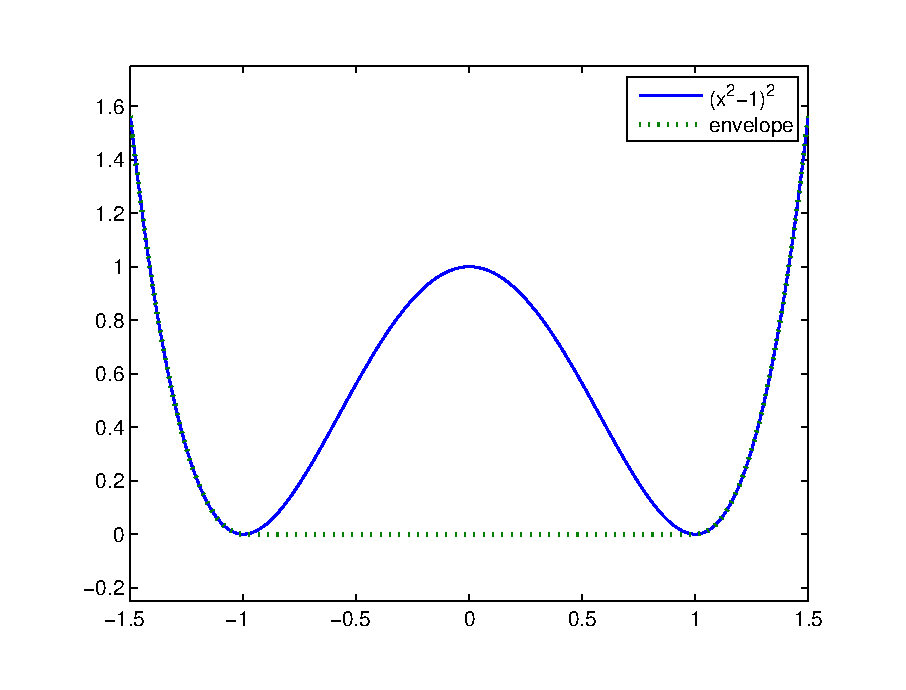
\includegraphics[width=4.5in]{envelope.eps}
\end{center}
~\\[-48pt]
\caption{The polynomial function $p(x)=x^4-2x^2+1$ and its convex envelope.}
\label{fig:envelope}
\end{figure}
The two coincide when $|x|\geq 1$, but deviate when $|x|<1$. Attempting to call
\verb@polyval([1,0,2,0,1],x)@ in a \cvx model would  yield an error,
but a call to \verb@poly_env([1,0,2,0,1],x)@ yields a valid 
representation of the envelope. For convex or concave polynomials,
this function produces the same result as \verb@polyval@.
\item \verb@pos@: $\max\{x,0\}$, for real $x$. 
Convex and increasing.
\item $\star$ \verb@pow_abs(x,p)@: $|x|^p$ for $x\in\R$ or $x\in\C$ and $p\geq 1$. Convex.
If \verb@p@ is irrational, a nearby rational value is chosen;
see Appendix \ref{sec:ratpow} for details.
\item $\star$ \verb@pow_pos(x,p)@: $\max\{x,0\}^p$ for $x\in\R$ and $p\geq 1$. Convex and
nondecreasing. If \verb@p@ is irrational, a nearby rational value is chosen;
see Appendix \ref{sec:ratpow} for details.
\item $\star$ \verb@pow_p(x,p)@, for $x\in\R$ and real constant $p$
computes nonnegative convex and concave branches of the power function:
\begin{equation*}
	\begin{aligned}
	&p \leq 0: \quad  
	f_p(x) &&\eqbydef \Cases{ x^p & x > 0 \\ +\infty & x \leq 0 } 
	&& \quad \text{convex, nonincreasing} \\
	0 <  &p \leq 1: \quad
	f_p(x) &&\eqbydef\Cases{ x^p & x \geq 0 \\ -\infty & x < 0 } 
	&& \quad  \text{concave, nondecreasing} \\
	&p \geq 1: \quad
	f_p(x) && \eqbydef\Cases{ x^p & x \geq 0 \\ +\infty & x < 0 }
	&& \quad \text{convex, nonmonotonic}
	\end{aligned}
\end{equation*}
\item \verb@quad_form(x,P)@, $x^TPx$ for real $x$ and symmetric $P$,
and $x^HPx$ for complex $x$ and Hermitian $P$.
Convex in $x$ for $P$ constant and positive semidefinite;
concave in $x$ for $P$ constant and negative semidefinite.
This function is provided since \cvx will \emph{not}
recognize \verb@x'*P*x@ as convex (even when \verb@P@ is 
positive semidefinite).
\item \verb@quad_over_lin@, $x^Tx/y$ for $x \in \R^n$, $y >0$;
for $x \in \complex^n$, $y>0$: $x^*x/y$.  In \cvx specification,
adds constraint that $y>0$.  Outside \cvx specification,
returns $+\infty$ if $y\leq 0$.
Convex, and decreasing in $y$.
\item \verb@quad_pos_over_lin@: \verb@sum_square_pos( x ) / y@
for $x\in\R^n$, $y>0$.
Convex, increasing in $x$, and decreasing in $y$.
%XXX \item \verb@rel_diff@, Relative (fractional) difference between 
%two numbers, $\max\{x/y, y/x\} -1$.  Inside \cvx, imposes constraint
%that $x$ and $y$ are positive.  Outside \cvx, returns $+\infty$
%if $x \leq 0$ or $y\leq 0$. Convex.
\item $\dagger$ \verb@rel_entr@: Scalar relative entropy: \verb@rel_entr(x,y)=x.*log(x/y)@. Convex.
\item \verb@sigma_max@: maximum singular value of real or 
complex matrix.  Same as \verb@norm@.  Convex.
\item \verb@square@: $x^2$ for $x \in \R$.
Convex.
\item \verb@square_abs@: $|x|^2$ for $x\in\R$ or $x\in\C$.
\item \verb@square_pos@: $\max\{x,0\}^2$ for $x\in\R$.
Convex and increasing.
\item \verb@sum_largest(x,k)@ sum of the largest $k$ values, for
real vector $x$.
Convex and increasing.
\item \verb@sum_smallest(x,k)@, sum of the smallest $k$ values,
\ie, \verb@-sum_smallest(-x,k)@.
Concave and decreasing.
\item \verb@sum_square@: \verb@sum( square( x ) )@. Convex.
\item \verb@sum_square_abs@: \verb@sum( square_abs( x ) )@. Convex.
\item \verb@sum_square_pos@: \verb@sum( square_pos( x ) )@; 
works only for real values. Convex and increasing.

\item \verb@trace_inv(X)@, trace of the inverse of an SPD matrix \verb@X@,
which is the same as the sum of the inverses of the eigenvalues.
Convex. 
Outside of \cvx, returns \verb@+Inf@ if argument is not positive definite.

\item \verb@trace_sqrtm(X)@, trace of the matrix squareroot of a positive
semidefinite matrix 
\verb@X@. which is the same as the sum of the squareroots of the 
eigenvalues.  Concave. 
Outside of \cvx, returns \verb@+Inf@ if argument is not positive semidefinite.
\end{itemize}

\iffalse
Functions to be added when smooth function support is added: 
\begin{itemize}
\item \verb@log_tsqr_minus_xsqr@: $\log (t^2-x^Tx)$
\item \verb@log_erf@: $\log \Phi$
\end{itemize}
\fi

\subsection{Sets}

\cvx currently supports the following sets; in each case, \verb@n@ is a positive
integer constant.
\begin{itemize}
\item \verb@nonnegative(n)@:
\begin{equation*}
	\reals^n_+ \eqbydef \Condset{x\in\Rn}{x_i\geq 0,~i=1,2,\dots,n}
\end{equation*}	
\item \verb@simplex(n)@:
\begin{equation*}
	\reals^n_{1+} \eqbydef \Condset{x\in\Rn}{x_i\geq 0,~i=1,2,\dots,n,~\TS\sum_ix_i=1}
\end{equation*}	
\item \verb@lorentz(n)@:
\begin{equation*}
\lorentz^n \eqbydef \Condset{(x,y)\in\R^n\times\R}{\|x\|_2\leq y}
\end{equation*}
\item \verb@rotated_lorentz(n)@: 
\begin{equation*}
\lorentz^n_r \eqbydef \Condset{(x,y,z)\in\R^n\times\R\times\R}{\|x\|_2\leq yz,~y,z\geq 0}
\end{equation*}
\item \verb@complex_lorentz(n):@ 
\begin{equation*}
\lorentz^n_c \eqbydef \Condset{(x,y)\in\complex^n\times\R}{\|x\|_2\leq y}
\end{equation*}
\item \verb@rotated_complex_lorentz(n)@: 
\begin{equation*}
\lorentz^n_{rc} \eqbydef \Condset{(x,y,z)\in\complex^n\times\R\times\R}{\|x\|_2\leq yz,~y,z\geq 0}
\end{equation*}
\item \verb@semidefinite(n):@ 
\begin{equation*}
\symm^n_+ \eqbydef \Condset{X\in\R^{n\times n}}{X=X^T,~X\succeq 0}
\end{equation*}
\item \verb@hermitian_semidefinite(n):@ 
\begin{equation*}
\herm^n_+ \eqbydef \Condset{Z\in\complex^{n\times n}}{Z=Z^H,~X\succeq 0}
\end{equation*}
\item \verb@nonneg_poly_coeffs(n):@ The cone of all coefficients of nonnegative
polynomials of degree $n$; $n$ must be even:
\begin{equation*}
\mathbf{P}_{+,n} \eqbydef \Condset{p\in\Rn[n+1]}{\sum_{i=0}^n p_{i+1} x^{n-i} \geq 0 ~ \forall x\in\R }
\end{equation*}
\item \verb@convex_poly_coeffs(n):@ The cone of all coefficients of convex
polynomials of degree $n$; $n$ must be even:
\begin{equation*}
\mathbf{P}_{+,n} \eqbydef \Condset{p\in\Rn[n+1]}{\sum_{i=0}^{n-2} (n-i)(n-i-1) p_{i+1} x^{n-i-2} \geq 0 ~ \forall x\in\R }
\end{equation*}
\item \verb@exponential_cone:@
\begin{equation*}
\mathbf{E} \eqbydef \text{cl}\Condset{(x,y,z)\in\R\times\R\times\R}{y>0,~ye^{x/y}\leq z}
\end{equation*}
\item \verb@geo_mean_cone(n)@:
\begin{equation*}
\mathbf{G}_n \eqbydef \text{cl}\Condset{(x,y)\in\Rn\times\Rn\times\Rn}{x\geq 0,~(\prod_{i=1}^n x_i)^{1/n} \geq y}
\end{equation*}
\end{itemize}

\newpage
\section{\cvx status messages}
\label{sec:status}
\index{status messages}
\index{cvx@{\cvx}!status messages}
\index{cvx@{\cvx}!precision}
\index{precision}

After a complete \cvx specification has been entered and the \verb@cvx_end@ command 
issued, the solver is called to generate a numerical result. The solver can produce
one of five exit conditions, which are indicated by the value of the string variable
\verb@cvx_status@. The nominal values of \verb@cvx_status@, and the resulting 
values of the other variables, are as follows:
\begin{itemize}
	\item \verb@Solved@: A complementary (primal and dual)
solution has been found.
	      The primal and dual variables are replaced with their computed values, and the
	      the optimal value of the problem is placed in \verb@cvx_optval@ (which, by
	      convention, is $0$ for feasibility problems).
	\item \verb@Unbounded@: The problem has been proven to be unbounded below
	      through the discovery of an unbounded primal direction. This direction
	      is stored in the primal variables. The value of \verb@cvx_optval@
	      is set to \verb@-Inf@ for minimizations, and
	      \verb@-Inf@ for maximizations. Feasibility problems by construction
	      cannot be unbounded below.
	      
	      It is important to understand that the unbounded primal direction is very
	      likely \emph{not} a feasible point. If a feasible point is required, the 
	      problem should be re-solved as a feasibility problem by omitting the objective.
	\item \verb@Infeasible@: The problem has been proven to be infeasible
	      through the discovery of an unbounded dual direction. Appropriate
	      components of this direction are stored in the dual variables. The values of the
	      primal variables are filled with \verb@NaN@s. The value of \verb@cvx_optval@
	      is set to \verb@+Inf@ for minimizations and feasibility problems,
	      and \verb@-Inf@ for maximizations.
\end{itemize}
In some cases, SeDuMi is unable to achieve the numerical certainty it requires to
make one of the above determinations---but is able to draw a weaker conclusion
by relaxing those tolerances somewhat. In such cases, one of the following
results is returned:
\begin{itemize}
	\item \verb@Inaccurate/Solved@: The problem is likely to have 
a complementary solution.
	\item \verb@Inaccurate/Unbounded@: The problem is likely to be unbounded.
	\item \verb@Inaccurate/Infeasible@: The problem is likely to be infeasible.
\end{itemize}
The values of the primal and dual variables, and of \verb@cvx_optval@, are updated
identically to the ``accurate'' cases. Two final results are also possible:
\begin{itemize}
	\item \verb@Failed@: The solver failed to make sufficient progress towards
	      a solution. The values of \verb@cvx_optval@ and primal and dual
	      variables are filled with \verb@NaN@s. This result can occur because
	      of numerical problems within SeDuMi, often because the problem
	      is particularly ``nasty'' in some way (\eg, a non-zero duality gap).
	\item \verb@Overdetermined@: The presolver has determined that the problem
	      has more equality constraints than variables, which means that the coefficient
	      matrix of the equality constraints is singular. In practice, such problems are
	      often, but not always, infeasible. Unfortunately, solvers 
	      typically cannot handle such problems, so a precise conclusion
	      cannot be reached.
\end{itemize}
The situations that most commonly produce an \verb@Overdetermined@ result are discussed
in \S\ref{sec:overdetermined} below.

\newpage
\section{Advanced solver topics}

\subsection{The successive approximation method}
\label{sec:succ-approx}
\index{successive approximation}
\index{cvx_expert@\texttt{cvx\_expert}}

Prior to version 1.2, the functions requested most often to be added to the 
\cvx function library were those from the exponential family,
including \verb@exp@, \verb@log@, and various
entropy functions. Unfortunately, \cvx utilizes symmetric primal/dual solvers 
that simply cannot support those functions natively; and a variety of practical
factors has delayed the use of other types of solvers with \cvx.

For this reason, we have constructed a \emph{successive approximation} method
that allows symmetric primal/dual solvers to support the exponential family
of functions. The precise nature of the method will be published elsewhere, but
we can provide a highly simplified description here. First, 
we construct a global approximation for \verb@exp@ (or \verb@log@,
\etc.) which is accurate within a neighborhood of some center point $x_0$.
Solving this approximation yields an approximate optimal point $\bar{x}$. We
shift the center point $x_0$ towards $\bar{x}$, construct a new approximation,
and solve again. This process is repeated until $|\bar{x}-x_0|$ is small enough to conclude
that our approximate is accurate enough to represent the original model.
Again, this is a highly simplified description of the approach; for instance, we
are also monitoring the dual problem as well to guide our judgements for shifting
$x_0$ and terminating.

\iffalse
So far, we have been quite pleased with the stability and accuracy of the successive 
approximation method. Nevertheless, we believe that the approach needs to be
tested further before it can be fully deployed, so \cvx ships with it
deactivated by default. To activate it, and thereby enable the use of functions
in the exponential family, insert the command
\begin{code}
cvx_expert true
\end{code}
into your model \emph{before} the \verb@cvx_begin@ command. 

Once we accumulate
wider experience with this approach, we will enable its use by default, and the
\verb@cvx_expert@ command will no longer be necessary (though we will leave it
in place for back-compatibility). In addition, we hope to find ways to integrate
the successive approximation method more tightly with the underlying solvers to
greatly improve its performance.
\fi

\iffalse
\subsection{The GP/SDP approximation}
\label{sec:gp-approx}
\index{precision!for GPs}
\index{cvx_gp_precision@\texttt{cvx\_gp\_precision}}

The solvers currently employed by \cvx does not support geometric programs natively.
Instead, \cvx \emph{approximates} the convex form of a DGP in an SDP-representable
manner. Details of the approximation method will be published separately; but in short,
it replaces each posynomial constraint with a series of polynomial
approximations. (Equalities and monomial inequalities do not require approximation.)

A key feature of this approximation method is that the error introduced at
each posynomial can be bounded in advance. Specifically,
given a constraint of the form
\begin{equation}
	\label{eq:constr-gp}
	f_i(x) \leq h_i(x) \quad f_i(x)\text{ posynomial, }h_i(x)\text{ monomial}
\end{equation}
the approximation produced by \cvx satisfies
\begin{equation}
	\label{eq:constr-approx}
	f_i(x) \cdot ( 1 + \delta_i ) \leq g_i(x), \quad \delta\in[0,\epsilon_{GP}]
\end{equation}
where $\delta_i$ is unknown but bounded as indicated.
The approximation is applied to posynomial objective functions as well. Thus
if the objective function is a posynomial $f_0(x)$, it will be perturbed to
$f_0(x)(1+\delta_0)$, where $\delta_0\in[0,\epsilon_{GP}]$. 

The approximations are \emph{conservative}, in that any value of $x$ that
satisfies an approximated constraint (\ref{eq:constr-approx})
will, in fact, satisfy the original (\ref{eq:constr-gp}) as well.
Applied to an entire DGP, this means that if \cvx locates a feasible point for
the approximated problem, that point is guaranteed to be feasible as well.
Furthermore, if \cvx successfully obtains an optimal value for the approximate
problem, that value will serve as an upper bound on the optimal value of
the original problem (for a minimization; for a maximization, it will serve
as a lower bound). 

In its default setting, \cvx uses a tolerance value of $\epsilon_{GP}=0.001$.
For most engineering applications, this is likely to be quite sufficient. However,
if you wish to change it, you may do so using the command
\verb@cvx_gp_precision(@\emph{tol}\verb@)@,
where \emph{tol} is the new value of $\epsilon_{GP}$. As with the command
\verb@cvx_precision@, you can place the call either within a model,
\begin{code}[commandchars=\!\{\}]
	cvx_begin gp
	    cvx_gp_precision(!textrm{!emph{tol}});
	    ...
	cvx_end
\end{code}
to change the approximation quality for a single model; or outside of a model,
\begin{code}[commandchars=\!\{\}]
	cvx_gp_precision(!textrm{!emph{tol}});
	cvx_begin gp
	    ...
	cvx_end
\end{code}
to make a global change. Consistent with
\cvx's other control commands, the command returns the \emph{previous}
value of the $\epsilon_{GP}$, so you can save it and restore it upon completion
of your model, if you wish. You can query the value of $\epsilon_{GP}$ at any
time by calling \verb@cvx_gp_precision@ with no arguments. 

It is important to understand that the complexity of the approximation---the order of
the polynomials used, as well as the number of them---increases as the
number of terms in the posynomial increases, and as the value of $\epsilon_{GP}$
decreases. Therefore, seeking high accuracies or solving problems involving 
posynomials with a vary large number terms can easily produce very large, slow
approximations.

This approximation can actually be used in DCPs as well.
Specifically, the function \verb@logsumexp_sdp@ uses this approximation
method to implement the function
\begin{equation}
	f:\Rn\rightarrow\R, \quad f(x) \eqbydef \log(\TS\sum_{i=1}^n e^{x_i}) + [0,\delta(x)], \quad \delta(x)\in[0,\epsilon]
\end{equation}
If you call this function directly, it uses a default tolerance of $\epsilon=0.001$, regardless
of the value set in \verb@cvx_gp_precision@. You can supply a different tolerance as a second
argument; \ie, \verb@logsumexp_sdp( x, tol )@.
\fi

\subsection{Irrational powers}
\label{sec:ratpow}
\index{powers}
\index{cvx_power_warning@\texttt{cvx\_power\_warning}}

In order to implement power expressions like $x^p$ and $p$-norms 
$\|x\|_p$ for $1<p<\infty$, \cvx uses an SDP-compatible method
described in \cite{Alizadeh}, and enhanced by the authors of \cvx.
This approach is exact---as long as the
exponent $p$ is rational. To determine integral values $p_n,p_d$ such
that $p_n/p_d=p$, \cvx
uses Matlab's \verb@rat@ function with its default tolerance
of $10^{-6}$. There is currently no way to change this tolerance.
See the documentation for \verb@rat@  for more details.

The complexity of the SDP implementation depends on roughly
on the size of the values $p_n$ and $p_d$. Let us introduce
a more precise measure of this complexity.
For $p=2$, a constraint $x^p\leq y$ can be represented with exactly
one $2\times 2$ LMI:
\begin{equation*}
	x^2 \leq y \quad\Longrightarrow\quad \bmat{ y & x \\ x & 1 } \succeq 0.
\end{equation*}
For other values of $p=p_n/p_d$, \cvx generates
a number of $2\times 2$ LMIs that depends on 
both $p_n$ and $p_d$; we denote this
number by $k(p_n,p_d)$. (A number of internal variables and
equality constraints are also
generated, but we ignore them for this analysis.) 
An empirical study has shown that for $p=p_n/p_d>1$, \cvx achieves
\begin{equation*}
k(p_n,p_d)\leq\log_2 p_n+\alpha(p_n),
\end{equation*}
where the  $\alpha(p_n)$ term
grows very slowly compared to the $\log_2$ term.
Indeed, for $p_n\leq 4096$, we have verified that $\alpha(p_n)$ is
usually 1 or 2, but occasionally 0 or 3.
Similar results are obtained for $0<p<1$ and $p<0$.

The cost of this SDP representation
is relatively small for nearly all useful values of $p$. Nevertheless,
\cvx issues a warning whenever $k(p_n,p_d)>10$ to insure that the user
is not surprised by any unexpected slowdown. In the event that this
threshold does not suit you, you may change it using the command
\verb@cvx_power_warning(@\emph{thresh}\verb@)@, where \emph{thresh}
is the desired cutoff value. Setting the
threshold to \verb@Inf@ disables it completely. 
As with the command \verb@cvx_precision@, you can place a
call to \verb@cvx_power_warning@ within a model
to change the threshold for a single model; or
outside of a model to make a global change. The command always
returns the \emph{previous}
value of the threshold, so you can save it and restore it upon completion
of your model, if you wish. You can query the current value
by calling \verb@cvx_power_warning@ with no arguments. 

\subsection{Overdetermined problems}
\label{sec:overdetermined}

\index{overdetermined problem}
\index{problem!overdetermined}
This status message \verb@Overdetermined@ commonly occurs when structure
in a variable or set is not properly recognized. For example, consider the problem
of finding the smallest diagonal addition to a matrix $W\in\Rnn$ to make it positive semidefinite:
\begin{equation}
	\begin{array}{ll}
		\text{minimize} & \mathop{\text{Trace}} D \\
		\text{subject to} & W + D \succeq 0 \\
		                  & D \text{~diagonal}
	\end{array}
\end{equation}
In \cvx, this problem might be expressed as follows:
\begin{code}
	n = size(W,1);
	cvx_begin
	    variable D(n,n) diagonal;
	    minimize( trace( D ) );
	    subject to
	        W + D == semidefinite(n);
	cvx_end
\end{code}
If we apply this specification to the matrix \verb@W=randn(5,5)@, a warning is issued,
\begin{code}
	Warning: Overdetermined equality constraints;
	    problem is likely infeasible.
\end{code}
and the variable \verb@cvx_status@ is set to \verb@Overdetermined@. 

What has happened here
is that the unnamed variable returned by statement \verb@semidefinite(n)@ is \emph{symmetric}, but
$W$ is fixed and \emph{unsymmetric}. Thus the problem, as stated, is infeasible. But
there are also $n^2$ equality constraints here, and only $n+n*(n+1)/2$ unique degrees
of freedom---thus the problem is overdetermined. The following modified 
version of the specification corrects this problem by extracting the symmetric part of $W$:
\begin{code}
	n = size(W,1);
	cvx_begin
	    variable D(n,n) diagonal;
	    minimize( trace( D ) );
	    subject to
	        0.5 * ( W + W' ) + D == semidefinite(n);
	cvx_end
\end{code}


\iffalse
\subsubsection{Defining new sets}
This version of \cvx does not support user-defined sets,
since we haven't yet settled on the best syntax.
This support will be added soon.

We can define new sets in \cvx in three basic ways, two of which
are supported in this first release.
The simplest is to use expressions and overloading, and the usual
function construction in Matlab.  But since only affine operations
can be applied to sets, this method cannot generate very 
interesting sets. 

The second method is analogous to specifying a convex or concave
function via an incomplete \cvx problem specification.
We describe a set by some constraints, given in \cvx form.
As an example, let's define a new set \verb@simplex(n)@, which is the
unit simplex in $\R^n$, defined as $\{x \in \R^n \;|\; 
x \succeq 0,~\ones^T x\leq 1 \}$.
To define this set, we create a file \verb@simplex.m@ containing
the following:
\begin{code}
function cvx_optval = simplex( n )
cvx_begin_set
variable x(n)
sum( x ) <= 1
x >= 0
cvx_end
\end{code}
We can now use this set in \cvx specifications.  For example, 
the line
\begin{code}
	A*x+b == simplex (size(A,1)) 
\end{code}
requires that $Ax+b$ must lie in the simplex of appropriate
dimension.
(Here we assume that \verb@x@ is a vector variable or affine
expression, and that \verb@A@ and \verb@b@ are a constant
matrix and vector, respectively, all of appropriate dimensions.

The one interesting twist is the use of the command 
\verb@cvx_begin_set@, instead of the usual \verb@cvx_begin@.
We can't use \verb@cvx_begin@ here, since the \cvx specification
above is \emph{complete}; it is interpreted as a feasibility problem.
If we used \verb@cvx_begin@ in this function, then when we call it,
\cvx forms the feasibility problem, discovers that it is complete,
and therefore solves it when it reaches the \verb@cvx_end@ command.
This problem is obivously feasible, so \verb@cvx_optval@ is \verb@0@,
so our function would simply always return \verb@0@.

XXX is it \verb@cvx_optval@ we want returned or \verb@x@?

The third method for defining a general convex set, with nonempty
interior, is to provide a barrier function (and its first and 
second derivatives) for the set.
This is not supported in the current version.
\fi

\iffalse
\subsection{Log-log-convex programming}

It is, in fact, possible to extend geometric programming beyond what is
described in \cite{BKVH:05} and in \S\ref{sec:gpmode}. 

GPs and GGPs are what we might call \emph{log-log-convex} optimization problems.
That is, in the same way that DCPs employ affine, convex, and concave functions
as building blocks, GPs and GGPs employ \emph{log-log-affine},
\emph{log-log-convex}, and \emph{log-log-concave} functions.
In short, a function $f:\Rn\rightarrow\R$
is log-log-affine (log-log-convex, log-log-concave) if
\begin{equation}
	\label{eq:log-log-affine}
	\tilde{f}:\Rn\rightarrow\R, \quad \tilde{f}(y) \eqbydef \log(f(\exp(y)))
\end{equation}
is affine (convex, concave), where
$\exp$ is an elementwise exponential function; \ie,
\begin{equation}
	\exp:\Rn\rightarrow\Rn_{++}, \quad 
	\exp(y) \eqbydef \bmat{e^{y_1} & \dots & e^{y_n}}^T.
\end{equation}
Monomials are log-log-affine and posynomials are log-log-convex, so
GPs are a protypical class of log-log-convex optimization problems.

The mapping $f\rightarrow\log\circ f\circ \exp$, which we will henceforth
call the \emph{log-log mapping}, can be used to create a nearly direct
translation of the rules in the DCP ruleset into a new set of rules in 
the log-log-convex ``domain.'' All standard GPs and GGPs satisfy these
rules; but so do many other problems as well.

It is not entirely clear that there are any \emph{useful}
log-log-convex problems which cannot be expressed in terms of a GP or GGP.
Until such examples are found, the ruleset will primarily be of academic
interest at best. But as a natural consequence of the implementation of GP mode,
\cvx supports log-log-convex programming. So we list the ruleset here.

\subsubsection{The log-curvature taxonomy}
\label{sec:gp-taxonomy}

For log-log-convex programming, three new categories of curvature are needed:
\emph{log-log-affine}, \emph{log-log-convex}, or \emph{log-log-concave}.
The categories contain those functions which are affine, convex,
and concave, respectively, after application of the log-log-mapping;
for example, $f$ is log-log-affine if $\log\circ f\circ\exp$ is affine.
The categories can, in fact, be described without the log-log transformation:
\begin{equation*}
\begin{array}{lc@{\,}lc}
\text{log-log-affine:}  & f(x^\alpha y^{1-\alpha}) & = f(x)^\alpha f(y)^{1-\alpha}& \forall x,y\in\Rn_+,~\alpha\in(0,1) \\
\text{log-log-convex:}  & \vdots & \leq        f(x)^\alpha f(y)^{1-\alpha} & \vdots \\
\text{log-log-concave:} &        & \geq        f(x)^\alpha f(y)^{1-\alpha} &
\end{array}
\end{equation*}
All expressions in these categories are real and nonnegative. As in the DCP case,
there is overlap between these categories; log-log-affine expressions are also
log-log-convex and log-log-concave. A log-log-affine
expression is always equivalent to a single monomial.
A posynomial is a log-log-convex expression, but posynomials cannot
represent the entire class. The class of log-log-concave expressions
(that are not also log-log-affine) is actually somewhat small, and is of limited usefulness;
nevertheless, the category is necessary for completeness.

\subsubsection{Constraints}
\label{sec:gp-constraints}

Three additional types of constraints may be specified in geometric problems:
\begin{itemize}
\item An \emph{equality constraint} \verb@==@ where both sides are log-log-affine expressions.
\item A \emph{less-than inequality constraint} \verb@<=@, \verb@<@ 
where the left side is log-log-convex and the right side is log-log-concave.
\item A \emph{greater-than inequality constraint} \verb@>=@, \verb@>@ 
where the left side is log-log-concave and the right side is log-log-convex.
\end{itemize}
Set membership constraints with log-log-affine arguments are acceptable as well.

\subsubsection{Expression rules}
\label{sec:gp-expressions}

The following are the rules for combining expressions from these new categories:
\begin{itemize}
\item A valid log-log-affine expression is
\begin{itemize}
\item a \emph{positive} (and, therefore, real) constant expression;
\item a declared geometric variable;
\item a valid call to a function in the atom library with a log-log-affine result;
\item the product of two or more log-log-affine expressions  (including cases where one or more are nonnegative constants);
\item the ratio of two log-log-affine expressions (including cases where either is a positive constant);
\item a log-log-affine expression raised to a real power;
\end{itemize}
\item A valid log-log-convex expression is
\begin{itemize}
\item a valid log-log-affine expression;
\item a valid call to a function in the atom library with a log-log-convex result;
\item the sum of two or more log-log-convex expressions;
\item the product of two or more log-log-convex expressions  (including cases where one or more are nonnegative constants);
\item the ratio of a log-log-convex expression and a log-log-concave expression (including cases where either is a positive constant);
\item a log-log-convex expression raised to a nonnegative real power;
\item a log-log-concave expression raised to a nonpositive real power.
\end{itemize}
\item A valid log-log-concave expression is
\begin{itemize}
\item a valid log-log-affine expression;
\item a valid call to a function in the atom library with a log-log-concave result;
\item the product of two or more log-log-concave expressions  (including cases where one or more are nonnegative constants);
\item the ratio of a log-log-concave expression and a log-log-convex expression (including cases where either is a positive constant);
\item a log-log-concave expression raised to a nonnegative real power;
\item a log-log-convex expression raised to a nonpositive real power.
\end{itemize}
\end{itemize}
It should not be difficult to see how each of these rules maps directly to a corresponding
rule in the DCP ruleset. For example, the rule permitting the sum of log-log-affine expressions
is the geometric counterpart to the rule permitting the \emph{sum} of affine expressions.
The sole omission from this ruleset, in fact, is the geometric equivalent of the scalar
quadratic form. On the other hand, the rules permitting sums of log-log-affine and
log-log-convex expressions do \emph{not} have counterparts in the DCP ruleset. They are
instead specific instances of the function composition rules; because in fact, 
summation is \emph{log-log-convex} in the geometric context.

\subsubsection{Functions and compositions}
\label{sec:gp-functions}

Disciplined geometric programming introduces three new categories 
for the curvature of functions: \emph{log-log-affine},
\emph{log-log-convex}, and \emph{log-log-concave}. Likewise,
three new categories of montonicity are introduced: \emph{p-nondecreasing},
\emph{p-nonincreasing}, and \emph{p-nonmonotonic}. The ``p-'' denotes
that the determination of monotonicity is made only over the nonnegative
orthant, instead of over the entire input space.
For example, a function $f:\Rn\rightarrow\R$ is p-nondecreasing if
\begin{equation}
	x \geq y \geq 0 \quad\Longrightarrow\quad f(x) \geq f(y)
\end{equation}
whereas the criteria for nondecreasing functions omits the nonnegativity test $\geq 0$.

The composition rules map over from DCP as you might expect:
\begin{itemize}
\item A log-log-convex, log-log-concave, or log-log-affine function may accept as an argument
a log-log-affine expression (assuming it is of compatible size).
\item If a function is log-log-convex and p-nondecreasing in a given argument,
then that argument may be log-log-convex.
\item If a function is log-log-convex and p-nonincreasing in a given argument,
then that argument may be log-log-concave.
\item If a function is log-log-concave and p-nondecreasing in a given argument,
then that argument may be log-log-concave.
\item If a function is log-log-concave and p-nonincreasing in a given argument,
then that argument may be log-log-convex.
\end{itemize}
(In each case, we assume that the argument is of compatible size.)

Here are some examples of DGP-compatible functions and their categorizations:
\begin{center}
\begin{tabular}{lll}
	\verb@prod( x )@    & $\prod_i x_i$& log-log-affine,  p-nondecreasing \\
	\verb@sum( x )@     & $\sum_i x_i$ & log-log-convex,  p-nondecreasing \\
	\verb@max( x, y )@  & $\max\{x,y\}$ & log-log-convex, p-nondecreasing \\
	\verb@min( x, y )@  & $\min\{x,y\}$ & log-log-concave, p-nondecreasing \\
	\verb@norm( x, p )@ & $\|x\|_p~(p\geq 1)$ & log-log-convex,  p-nondecreasing \\ 
	\verb@sqrt( x )@    & $x^{1/2}$    & log-log-affine, p-nondecreasing \\
	\verb@1/x@          & $x^{-1}$     & log-log-affine, p-nonincreasing
\end{tabular}
\end{center}
For instance, if \verb@x@, \verb@y@, and \verb@z@ are scalar geometric variables, then
\begin{code}
	max( x + y, y + z ^ 2 )
\end{code}
is log-log-convex, because the posynomial arguments are log-log-convex, and \verb@max@ is log-log-convex
and p-nondecreasing. 

Clearly, a function that is monotonic is also p-monotonic in the same sense;
for example, \verb@sum@ is both nondecreasing and p-nondecreasing. The
reverse implication is \emph{not} true; for example,
\verb@norm( x, q )@ is p-nondecreasing in x, but nonmonotonic.
\fi

\section{Acknowledgements}

We wish to thank the following people for their contributions to
the development of \cvx: Toh Kim Chuan, Laurent El Ghaoui, Arpita Ghosh, 
Siddharth Joshi, Johan L\"{o}fberg, Almir Mutapcic, Michael Overton
and his students, Art Owen, Rahul Panicker, Imre Polik, Jo\"{e}lle Skaf, 
Lieven Vandenberghe, Argyris Zymnis. We are also grateful to the many
students in several universities who have (perhaps unwittingly)
served as beta testers by using \cvx in their classwork.
We thank Igal Sason for catching many typos in an earlier version of this 
document, and generally helping us to improve its clarity.

\newpage
\bibliography{cvx_usrguide}
\newpage
\printindex
\end{document}
